\documentclass[a4paper, 12pt]{book}

% Packages
\usepackage[utf8]{inputenc} % Input encoding
\usepackage[T1]{fontenc}    % Font encoding
\usepackage[margin=1in]{geometry} % Adjust margins
\usepackage{titling}        % Custom title format
% \usepackage{fancyhdr}       % Custom headers and footers
\usepackage{amsmath,amsfonts,amssymb}
\usepackage[english]{babel}
\usepackage{mathtools}
\usepackage{xcolor}
\usepackage{mdframed}

% \pagestyle{fancy}
% Remove indentation at the beginning of a paragraph
\setlength{\parindent}{0pt}
% Title
\title{Notes for Numerical Methods}
\date{\today}

\begin{document}
\maketitle
% \chapter[short]{Matrix Algebra}


\[
A = \begin{pmatrix}
a_{11} & a_{12} & \cdots & a_{1m} \\
a_{21} & a_{22} & \cdots & a_{2m} \\
\vdots & \vdots & \ddots & \vdots \\
a_{m1} & a_{m2} & \cdots & a_{mm}
\end{pmatrix}
\]
If every element in $A$ is a real number, we write $A \in \mathbb{R}^{m \times m}$ where $m$ is the number of rows and $n$ is the number of columns.

If every element in $A$ is a complex number, we write $A \in \mathbb{C}^{m \times m}$.

With matrices, we can perform some operations.

\section{Matrix Algebra}

\subsection{Addition}
Given two matrices of the same size $A$ and $B$:
\begin{itemize}
    \item $C = A + B$ \quad $c_{ij} = a_{ij} + b_{ij}$
    \item $C = -A$ \quad $c_{ij} = -a_{ij}$
    \item $C = A - B$ \quad $c_{ij} = a_{ij} - b_{ij}$
\end{itemize}

\textbf{Properties}
\begin{itemize}
    \item Closure:
    \begin{quote}
    Given $A, B \in \mathbb{R}^{m \times m}$, then if $C = A + B$ \\
    $\Rightarrow C \in \mathbb{R}^{m \times m}$.
    \end{quote}
    
    \item Associative:
    \begin{equation*}
    (A + B) + C = A + (B + C)
    \end{equation*}
    
    \item Additive Identity:
    \begin{equation*}
    A + O = A = O + A
    \end{equation*}
\end{itemize}

\section{Matrix Properties}
\section{Note:}
\textbf{O} is the matrix with all 0 elements.

\begin{enumerate}
    \item \textbf{Additive inverse}
    \[ A + (-A) = O \]
    
    \item \textbf{Multiplication with a scalar}
    \[ \alpha \in \mathbb{R} \]
    \[ C = \alpha A \]
    \[ c_{ij} = \alpha a_{ij} \quad \text{(element-wise multiplication)} \]
    
    \textbf{Properties}
    \begin{itemize}
        \item \textbf{Closure}
        \[ \alpha \in \mathbb{R}, \ A \in \mathbb{R}^{m \times m} \]
        \[ \text{If } C = \alpha A \Rightarrow C \in \mathbb{R}^{m \times m} \]
        
        \item \textbf{Associative}
        \[ \alpha, \beta \in \mathbb{R}, \ A \in \mathbb{R}^{m \times m} \]
        \[ (\alpha \beta) A = \alpha (\beta A) \]
        
        \item \textbf{Distributive over matrix addition}
        \[ \alpha (A + B) = \alpha A + \alpha B \]
    \end{itemize}
\end{enumerate}





\section{Matrix Properties and Transpose}

\textbf{Distributive over scalar addition:}
\[(\alpha + \beta) \mathbf{A} = \alpha \mathbf{A} + \beta \mathbf{A}\]

\textbf{Identity:}
\[I \cdot \mathbf{A} = \mathbf{A}\]

\textit{Note:} $I$ is a matrix with elements equal to 1.

\section{Transpose Matrix}

Given $\mathbf{A}$ "square", it means the number of rows is equal to the number of columns. For example, $\mathbf{A} \in \mathbb{R}^{m \times m}$, the \textbf{TRANSPOSE} is denoted by the symbol $\mathbf{A}^T$ and it is constructed by exchanging the rows and the columns of $\mathbf{A}$.

\textbf{Example:}

\[
\mathbf{A} = 
\begin{bmatrix}
1 & 2 \\
3 & 4
\end{bmatrix}
\]

\[
\mathbf{A}^T = 
\begin{bmatrix}
1 & 3 \\
2 & 4
\end{bmatrix}
\]

\section{Special Matrices}





If $C = A^T$ then $c_{ij} = a_{ji}$.

\textbf{Note:}
\[(A^T)^T = A\]

If a given square matrix $A$ is equal to its transpose, $A$ is said to be \textbf{symmetric}.

If
\[A = A^T\]
then $A$ is symmetric.

Example:
\[A = \begin{pmatrix}
1 & 2 \\
2 & 1
\end{pmatrix}\]

Therefore,
\[A = \begin{pmatrix}
1 & 2 & 3 \\
2 & 4 & 5 \\
3 & 5 & 6
\end{pmatrix}\]

If $A = -A^T$ then $A$ is said to be \textbf{skew-symmetric}.

\section{Special Matrices}


\section{Identity Matrix}
The identity matrix is usually denoted with $I$ and it has 1 on the main diagonal and 0 everywhere else.
\[
I = \begin{pmatrix}
1 & 0 & \cdots & 0 \\
0 & 1 & \cdots & 0 \\
\vdots & \vdots & \ddots & \vdots \\
0 & 0 & \cdots & 1
\end{pmatrix}
\]
The identity matrix is such that
\[
AI = IA = A
\]

\section{Triangular Matrices}
\subsection*{Upper Triangular}
An upper triangular matrix $A$ is of the form:
\[
A = \begin{pmatrix}
a_{11} & a_{12} & \cdots & a_{1n} \\
0 & a_{22} & \cdots & a_{2n} \\
\vdots & \vdots & \ddots & \vdots \\
0 & 0 & \cdots & a_{nn}
\end{pmatrix}
\]
Only the elements above the main diagonal and the diagonal elements are $\neq 0$.





\section{Lower Triangular Matrices}
A lower triangular matrix $A$ is given by:
\[
A = \begin{pmatrix}
a_{11} & 0 & \cdots & 0 \\
a_{21} & a_{22} & \cdots & 0 \\
\vdots & \vdots & \ddots & \vdots \\
a_{m1} & a_{m2} & \cdots & a_{mm}
\end{pmatrix}
\]
Only the elements below the main diagonal and the diagonal elements are $\neq 0$.

\section{Diagonal Matrices}
A diagonal matrix $A$ is given by:
\[
A = \begin{pmatrix}
a_{11} & 0 & \cdots & 0 \\
0 & a_{22} & \cdots & 0 \\
\vdots & \vdots & \ddots & \vdots \\
0 & 0 & \cdots & a_{mm}
\end{pmatrix}
\]
Only the elements on the main diagonal are $\neq 0$.

\section{Matrix Product}
Given $A \in \mathbb{R}^{n \times p}$, $B \in \mathbb{R}^{p \times m}$, the product $AB$ is possible because the two matrices are said \textit{conformable}: the number of columns of the first matrix should be equal to the number of rows of the second matrix.



Equal the number of rows of the second matrix. The resulting matrix $C = AB$ has the size $m \times n$.

Example
\[
A = \begin{pmatrix}
1 & 2 \\
3 & 4
\end{pmatrix}
\quad
B = \begin{pmatrix}
3 & 1 \\
1 & 2
\end{pmatrix}
\]

\[
C = AB = \begin{pmatrix}
c_{11} & c_{12} \\
c_{21} & c_{22}
\end{pmatrix}
=
\begin{pmatrix}
1\cdot3 + 2\cdot1 & 1\cdot1 + 2\cdot2 \\
3\cdot3 + 4\cdot1 & 3\cdot1 + 4\cdot2
\end{pmatrix}
=
\begin{pmatrix}
5 & 5 \\
13 & 11
\end{pmatrix}
\]

\[
c_{11} = a_{11}b_{11} + a_{12}b_{21}
\]
\[
c_{12} = a_{11}b_{12} + a_{12}b_{22}
\]
\[
c_{21} = a_{21}b_{11} + a_{22}b_{21}
\]
\[
c_{22} = a_{21}b_{12} + a_{22}b_{22}
\]

\[
\boxed{
c_{ij} = \sum_{k=1}^{m} a_{ik}b_{kj}
}
\]

\[
c_{11} = a_{11}b_{11} + a_{12}b_{21}
\]
\[
c_{12} = a_{11}b_{12} + a_{12}b_{22}
\]

\section{Matrix Multiplication}




\section{Matrix Multiplication Properties}

\begin{itemize}
    \item The matrix product is \textbf{not commutative}:
    \[ AB \neq BA \]

    \item For scalars $\alpha, \beta \in \mathbb{R}$ when $\alpha\beta = 0$:
    \[ \text{either } \alpha = 0 \text{ or } \beta = 0 \text{ or } \alpha\beta = 0 \]

    \item For matrices $A, B$ consider the case when $AB = O$ (the zero matrix). It could be that:
    \[ A \neq O \text{ and } B \neq O \]

    \item Example:
    \[ A = \begin{pmatrix} 1 & 1 \\ 1 & 1 \end{pmatrix}, \quad B = \begin{pmatrix} 2 & 2 \\ -2 & -2 \end{pmatrix} \]
    \[ AB = \begin{pmatrix} 0 & 0 \\ 0 & 0 \end{pmatrix} \]

    \item The ``cancellation law'' does not hold for matrices. For scalars $\alpha, \beta, \gamma \in \mathbb{R}$:
\end{itemize}



If $\alpha \beta = \alpha \gamma$ and $\alpha \neq 0$ \\
then $\beta = \gamma$.

\[
A = \begin{pmatrix}
1 & 1 \\
1 & 1
\end{pmatrix}, \quad
B = \begin{pmatrix}
2 & 2 \\
2 & 2
\end{pmatrix}, \quad
C = \begin{pmatrix}
3 & 1 \\
1 & 3
\end{pmatrix}.
\]

\[
AB = \begin{pmatrix}
4 & 4 \\
4 & 4
\end{pmatrix} = AC \text{ but } B \neq C.
\]

\textbf{The matrix product is a linear function.}

Given a function $f: \mathbb{R} \to \mathbb{R}$ it is said to be linear if

\begin{enumerate}
\item $\forall x_1, x_2 \in \mathbb{R}$ \\
$f(x_1 + x_2) = f(x_1) + f(x_2)$
\item $\forall \alpha \in \mathbb{R}$ \\
$\alpha f(x) = f(\alpha x)$
\end{enumerate}

\section{Linearity of Functions}





\section{Example}
Consider the function $f(x) := 3x$ where $f: \mathbb{R} \to \mathbb{R}$.

\textbf{Is $f$ linear?}

Let's see if the two conditions of linearity are satisfied:

\begin{enumerate}
    \item For all $x_1, x_2 \in \mathbb{R}$, is the following condition satisfied?
    \[ f(x_1 + x_2) \stackrel{?}{=} f(x_1) + f(x_2) \]
    We have:
    \begin{align*}
        f(x_1 + x_2) &= 3(x_1 + x_2) \\
        &= 3x_1 + 3x_2 \\
        &= f(x_1) + f(x_2)
    \end{align*}
    Yes! Due to the distributive property.

    \item For all $\alpha \in \mathbb{R}$, is the following condition satisfied?
    \[ \alpha f(x) \stackrel{?}{=} f(\alpha x) \]
    We have:
    \begin{align*}
        \alpha f(x) &= \alpha(3x) \\
        &= 3\alpha x \\
        &= f(\alpha x)
    \end{align*}
    Yes! Commutative property.
    
    Therefore, $f$ is a linear function.
\end{enumerate}

Thus, this example is clear that any function $f: \mathbb{R} \to \mathbb{R}$ defined as $f(x) := \alpha x$ with $\alpha \in \mathbb{R}$ is linear.

\section{Linear Functions}




A function $f: \mathbb{R} \to \mathbb{R}$ is called a \textbf{linear function} if it can be expressed in the form $f(x) = \alpha x + \beta$ with $\alpha, \beta \in \mathbb{R}$ and $\beta \neq 0$. 

\textbf{Example:}

Consider the function $f: \mathbb{R} \to \mathbb{R}$ defined by $f(x) = \alpha x + \beta$ with $\alpha, \beta \in \mathbb{R}$ and $\beta \neq 0$. Is $f$ linear?

To determine if $f$ is linear, we check if for all $x_1, x_2 \in \mathbb{R}$, the following property holds:
\[
f(x_1 + x_2) \stackrel{?}{=} f(x_1) + f(x_2)
\]
Starting with the left-hand side:
\[
f(x_1 + x_2) = \alpha(x_1 + x_2) + \beta = \alpha x_1 + \alpha x_2 + \beta
\]
And the right-hand side:
\[
f(x_1) + f(x_2) = (\alpha x_1 + \beta) + (\alpha x_2 + \beta) = \alpha x_1 + \alpha x_2 + 2\beta
\]
Since $\alpha x_1 + \alpha x_2 + \beta \neq \alpha x_1 + \alpha x_2 + 2\beta$, $f$ is \textbf{not linear}.

This type of function is called an \textbf{affine function}.

\textbf{Example:}

The function \textit{Differentiation} is a linear function.

\section{Differentiation and Integration Rules}




\section{Differentiation}
Given two functions of \( x \), \( f \) and \( g \):
\[ f, g : \mathbb{R} \to \mathbb{R} \]
\[ \frac{d}{dx} (f + g) = \frac{df}{dx} + \frac{dg}{dx} \]
\[ \frac{d}{dx} (\alpha \cdot f) = \alpha \cdot \frac{df}{dx} \]

\section{Integration}
\[ f, g : \mathbb{R} \to \mathbb{R} \]
\[ \int (f + g) = \int f + \int g \]
\[ \int \alpha f = \alpha \int f \]

\section{Transpose}
\[ \text{For matrices } A \text{ and } B \text{ in } \mathbb{R}^{m \times m} \]
\[ (A + B)^T = A^T + B^T \]
\[ (\alpha A)^T = \alpha A^T \]

\section{Trace of a Matrix}





Given a matrix $A$ with elements $a_{ij}$, the trace of $A$ is the sum of the elements on the main diagonal:
\[
\text{Trace}(A) := \sum_i a_{ii}
\]

The trace of a matrix is a linear function:
\begin{enumerate}
    \item $\text{Trace}(A + B) = \text{Trace}(A) + \text{Trace}(B)$
    \[
    \sum_i (a_{ii} + b_{ii}) = \sum_i a_{ii} + \sum_i b_{ii} \quad \text{Yes!}
    \]
    
    \item $\text{Trace}(\alpha A) = \alpha \text{Trace}(A)$
    \[
    \sum_i \alpha a_{ii} = \alpha \sum_i a_{ii}.
    \]
\end{enumerate}

\textbf{Example}

Let $f: \mathbb{R}^2 \to \mathbb{R}^2$ be defined by
\[
f\left(\begin{array}{c}
    x \\
    y
\end{array}\right) := \left(\begin{array}{c}
    x \\
    x + y
\end{array}\right).
\]

\section{Is $f$ linear?}




Let $v, w \in \mathbb{R}^2$ with $v = \begin{pmatrix} v_1 \\ v_2 \end{pmatrix}$ and $w = \begin{pmatrix} w_1 \\ w_2 \end{pmatrix}$.

Is it true that $f(v + w) = f(v) + f(w)$?

\begin{align*}
f(v + w) &= f\left( \begin{pmatrix} v_1 \\ v_2 \end{pmatrix} + \begin{pmatrix} w_1 \\ w_2 \end{pmatrix} \right) \\
&= f\left( \begin{pmatrix} v_1 + w_1 \\ v_2 + w_2 \end{pmatrix} \right) \\
&= \begin{pmatrix} v_1 + w_1 \\ 1 + v_2 + w_2 \end{pmatrix} \\
f(v) + f(w) &= f\left( \begin{pmatrix} v_1 \\ v_2 \end{pmatrix} \right) + f\left( \begin{pmatrix} w_1 \\ w_2 \end{pmatrix} \right) \\
&= \begin{pmatrix} v_1 \\ 1 + v_2 \end{pmatrix} + \begin{pmatrix} w_1 \\ 1 + w_2 \end{pmatrix} \\
&= \begin{pmatrix} v_1 + w_1 \\ 1 + v_2 + 1 + w_2 \end{pmatrix} \\
&= \begin{pmatrix} v_1 + w_1 \\ 1 + v_2 + w_2 + 1 \end{pmatrix}
\end{align*}

Thus, $f$ is not linear as $f(v + w) \neq f(v) + f(w)$.




Example:
\[
f\left( \begin{array}{c}
x \\
y
\end{array} \right) := \left( \begin{array}{c}
0 \\
xy
\end{array} \right) \quad f: \mathbb{R}^2 \to \mathbb{R}^2
\]

Is $f$ linear?

Let $\mathbf{v}, \mathbf{w} \in \mathbb{R}^2$

$\mathbf{v} = \left( \begin{array}{c}
v_1 \\
v_2
\end{array} \right)$, $\mathbf{w} = \left( \begin{array}{c}
w_1 \\
w_2
\end{array} \right)$

\[
f(\mathbf{v} + \mathbf{w}) \stackrel{?}{=} f(\mathbf{v}) + f(\mathbf{w})
\]

\[
f(\mathbf{v} + \mathbf{w}) = f\left( \begin{array}{c}
v_1 + w_1 \\
v_2 + w_2
\end{array} \right) = \left( \begin{array}{c}
0 \\
(v_1 + w_1)(v_2 + w_2)
\end{array} \right)
\]

\[
= \left( \begin{array}{c}
0 \\
v_1v_2 + v_1w_2 + w_1v_2 + w_1w_2
\end{array} \right)
\]

\[
f(\mathbf{v}) + f(\mathbf{w}) = f\left( \begin{array}{c}
v_1 \\
v_2
\end{array} \right) + f\left( \begin{array}{c}
w_1 \\
w_2
\end{array} \right)
\]

\[
= \left( \begin{array}{c}
0 \\
v_1v_2
\end{array} \right) + \left( \begin{array}{c}
0 \\
w_1w_2
\end{array} \right) = \left( \begin{array}{c}
0 \\
v_1v_2 + w_1w_2
\end{array} \right)
\]

\section{Exercise Set}
$f$ is not linear as $f(x+y) \neq f(x) + f(y)$.

\section{Exercises:}
Refer book, page 92, exercise 3.3.1

\section{Composition of 2 functions.}
\[
f\begin{pmatrix}
x_1 \\
x_2
\end{pmatrix}
:=
\begin{pmatrix}
f_{11}x_1 + f_{12}x_2 \\
f_{21}x_1 + f_{22}x_2
\end{pmatrix}
\]

\[
g\begin{pmatrix}
x_1 \\
x_2
\end{pmatrix}
:=
\begin{pmatrix}
g_{11}x_1 + g_{12}x_2 \\
g_{21}x_1 + g_{22}x_2
\end{pmatrix}
\]

We define $h$ the composition of $f$ and $g$ using symbols
\[
h(x) = f(g(x)) \quad \text{where} \quad x = \begin{pmatrix}
x_1 \\
x_2
\end{pmatrix}
\]

\[
h(x) = h\begin{pmatrix}
x_1 \\
x_2
\end{pmatrix}
=
f\begin{pmatrix}
g_{11}x_1 + g_{12}x_2 \\
g_{21}x_1 + g_{22}x_2
\end{pmatrix}
\]

\begin{align*}
&= \left\{
\begin{array}{cc}
f_{11} g_{11} x_1 + f_{12} g_{21} x_2 & + f_{12} g_{21} x_1 + f_{22} g_{22} x_2 \\
f_{21} (g_{11} x_1 + g_{12} x_2) & + f_{22} (g_{21} x_1 + g_{22} x_2)
\end{array}
\right. \\
&= \left\{
\begin{array}{c}
f_{11} g_{11} x_1 + f_{12} g_{21} x_2 + f_{12} g_{21} x_1 + f_{22} g_{22} x_2 \\
f_{21} g_{11} x_1 + f_{21} g_{12} x_2 + f_{22} g_{21} x_1 + f_{22} g_{22} x_2
\end{array}
\right. \\
&= \left\{
\begin{array}{c}
(f_{11} g_{11} + f_{12} g_{21}) x_1 + (f_{12} g_{21} + f_{22} g_{22}) x_2 \\
(f_{21} g_{11} + f_{22} g_{21}) x_1 + (f_{21} g_{12} + f_{22} g_{22}) x_2
\end{array}
\right. \\
\text{Let us introduce the following matrices} \\
T &:= \begin{pmatrix}
f_{11} & f_{12} \\
f_{21} & f_{22}
\end{pmatrix}; \quad G := \begin{pmatrix}
g_{11} & g_{12} \\
g_{21} & g_{22}
\end{pmatrix} \\
H &:= TG = \begin{pmatrix}
f_{11} g_{11} + f_{12} g_{21} & f_{11} g_{12} + f_{12} g_{22} \\
f_{21} g_{11} + f_{22} g_{21} & f_{21} g_{12} + f_{22} g_{22}
\end{pmatrix}
\end{align*}\section{The Vector Space of Continuous Functions}





The vector space of continuous functions can be seen as the composition of two linear functions.

\textbf{Note:} To check for "linearity" we can use a general process which includes the two conditions:

\begin{align*}
f: \mathbb{R}^n &\to \mathbb{R} \\
\forall x, y \in \mathbb{R}^n \text{ and } \forall \alpha \in \mathbb{R}, \text{ if} \\
f(\alpha x + y) &= \alpha f(x) + f(y) \\
\text{then } f &\text{ is said to be linear.}
\end{align*}

\section{BLOCK MATRICES}

\[
A = \begin{pmatrix}
1 & 2 & 0 & 0 \\
3 & 4 & 0 & 1 \\
-1 & 0 & 0 & 0 \\
0 & 1 & 0 & 0
\end{pmatrix}
\qquad
C = \begin{pmatrix}
1 & 2 \\
3 & 4
\end{pmatrix}
\]

\begin{align*}
B &= \begin{pmatrix}
1 & 0 & 0 & 0 \\
0 & 1 & 0 & 0 \\
\frac{1}{3} & \frac{2}{3} & \frac{1}{3} & \frac{2}{3} \\
\frac{1}{3} & \frac{2}{3} & \frac{1}{3} & \frac{2}{3}
\end{pmatrix} \\[10pt]
\text{We can rewrite } A \text{ and } B \text{ as:} \\[10pt]
A &= \begin{pmatrix}
C & I \\
I & O
\end{pmatrix} \\[10pt]
B &= \begin{pmatrix}
I & O \\
C & C
\end{pmatrix} \\[10pt]
AB &= \begin{pmatrix}
C & I \\
I & O
\end{pmatrix}
\begin{pmatrix}
I & O \\
C & C
\end{pmatrix} \\[10pt]
&= \begin{pmatrix}
CI + IC & CO + IC \\
I + OC & IO + OC
\end{pmatrix}
\end{align*}\begin{equation*}
\begin{pmatrix}
2C \\
I
\end{pmatrix}
\quad
\begin{pmatrix}
C \\
O
\end{pmatrix}
\quad = \quad
\begin{pmatrix}
2 & 4 & 1 & 2 \\
6 & 8 & 3 & 4 \\
4 & 0 & 0 & 0 \\
0 & 1 & 0 & 0
\end{pmatrix}
\end{equation*}

\textbf{example}

\begin{equation*}
A = 
\begin{pmatrix}
4 & 0 & 0 & 3 & 3 & 3 \\
1 & 0 & 0 & 3 & 3 & 3 \\
1 & 2 & 0 & 0 & 0 & 0
\end{pmatrix}
\quad = \quad
\begin{pmatrix}
A_{11} & A_{12} & A_{13} \\
A_{21} & A_{22} & A_{23}
\end{pmatrix}
\quad
\begin{matrix}
2 \times 3 \text{ block}
\end{matrix}
\end{equation*}

\begin{equation*}
B = 
\begin{pmatrix}
-1 & -1 \\
0 & 0 \\
1 & -2 \\
1 & -2
\end{pmatrix}
\quad = \quad
\begin{pmatrix}
B_{1} \\
B_{2} \\
B_{3}
\end{pmatrix}
\quad
\begin{matrix}
3 \times 1 \text{ blocks}
\end{matrix}
\end{equation*}\section{Matrix Multiplication}




\section{Matrix Product $AB$}
Given two matrices $A$ and $B$:
\[ AB = \begin{pmatrix}
A_{11} & A_{12} & A_{13} \\
A_{21} & A_{22} & A_{23}
\end{pmatrix}
\begin{pmatrix}
B_1 \\
B_2 \\
B_3
\end{pmatrix}
\]

The product is computed as:
\[
\begin{aligned}
& A_{11} B_1 + A_{12} B_2 + A_{13} B_3 \\
& A_{21} B_1 + A_{22} B_2 + A_{23} B_3
\end{aligned}
\]

\section{Component-wise Multiplication}
Now we perform the component-wise multiplication step by step.

\[
A_{11} B_1 = \begin{pmatrix}
1 \\
1
\end{pmatrix}
\begin{pmatrix}
-1 & -1
\end{pmatrix}
= \begin{pmatrix}
-1 & -1 \\
-1 & -1
\end{pmatrix}
\]

\[
A_{12} B_2 = \begin{pmatrix}
0 & 0 \\
0 & 0
\end{pmatrix}
\begin{pmatrix}
0 & 0
\end{pmatrix}
= \begin{pmatrix}
0 & 0 \\
0 & 0
\end{pmatrix}
\]

\[
A_{13} B_3 = \begin{pmatrix}
3 & 3 & 3 \\
3 & 3 & 3
\end{pmatrix}
\begin{pmatrix}
-1 \\
-2 \\
-1
\end{pmatrix}
= \begin{pmatrix}
-9 & -9 \\
-9 & -9
\end{pmatrix}
\]

\[
A_{21} B_1 = 1 \cdot \begin{pmatrix}
-1 & -1
\end{pmatrix}
= \begin{pmatrix}
-1 & -1
\end{pmatrix}
\]

\[
A_{22} B_2 = \begin{pmatrix}
0 & 0
\end{pmatrix}
\begin{pmatrix}
0 & 0
\end{pmatrix}
= \begin{pmatrix}
0 & 0
\end{pmatrix}
\]

\section{Matrix Operations}
\[
A_{23} B_{3} = \begin{pmatrix}
0 & 0 \\
-1 & -1
\end{pmatrix}
\]

\[
\begin{pmatrix}
-1 & -1 \\
-1 & -1
\end{pmatrix}
+ \begin{pmatrix}
0 & 0 \\
0 & 0
\end{pmatrix}
+ \begin{pmatrix}
-9 & -18 \\
-9 & -18
\end{pmatrix}
\]

\[
= \begin{pmatrix}
-1 & -1 \\
-1 & -1
\end{pmatrix}
+ \begin{pmatrix}
0 & 0 \\
0 & 0
\end{pmatrix}
+ \begin{pmatrix}
0 & 0 \\
0 & 0
\end{pmatrix}
\]

\[
= \begin{pmatrix}
-1 & -1 \\
-1 & -1
\end{pmatrix}
+ \begin{pmatrix}
-19 & -19 \\
-19 & -19
\end{pmatrix},
\]

\subsection{Notes}
\begin{itemize}
\item Check example 3.6.7 from Mayer book for block triangular matrices and simultaneous causality.
\item Application to airline connectivity (see example 3.5.2 from Mayer book).
\item Let us consider the following 5 cities: A, B, C, D, H.
\end{itemize}

\section{Graph Theory: Adjacency Matrix}




The arrows tell us which cities are connected with a \textbf{direct flight}.

We want to represent how city $A$ is city $B$ and consider only the routes with 3 flights.

\begin{itemize}
    \item $A - H - D - B$
    \item $A - C - H - B$
    \item $A - C - D - B$
\end{itemize}

To model this problem we construct the so-called \textbf{ADJACENCY MATRIX} $C$ (or \textbf{connectivity}).

\[
c_{ij} = 
\begin{cases} 
1 & \text{if there is a direct flight from city $i$ to city $j$} \\
0 & \text{otherwise}
\end{cases}
\]

\section{Flight Connectivity Matrix}




The matrix $C$ represents the connectivity between cities:

\[
C = \begin{pmatrix}
0 & 0 & 1 & 0 & 1 \\
1 & 0 & 0 & 0 & 1 \\
0 & 0 & 0 & 1 & 1 \\
1 & 0 & 0 & 0 & 1 \\
1 & 1 & 1 & 0 & 0 \\
\end{pmatrix}
\]

\begin{itemize}
    \item The number $c_{ik}$ states if there is a direct flight from city $i$ to city $k$.
    \item The number $c_{kj}$ states if there is a direct flight from city $k$ to city $j$.
    \item The number of flight routes between city $i$ and city $j$ passing through city $k$ is given by $c_{ik} \cdot c_{kj}$.
    \item The total number of flight routes between city $i$ and city $j$ is then
    \[
    \sum_{k} c_{ik} \cdot c_{kj}
    \]
\end{itemize}



We can recursively compute this for all the cities as \( C \cdot C = C^2 \).

We want to show that \( C^m \) gives us the total number of \( m \)-flights routes between the cities in our network.

The proof is shown by using the "induction principle".

\begin{enumerate}
    \item BASIC STEP: \( m = 1 \) \(\Rightarrow\) \( C^1 = C \) \\
    By construction gives us the number of 1-flight routes between the cities.
    
    \item We assume the statement to be true when \( m = (m-1) \), then we move it for the next step:
    
    Suppose that \( C^{(m-1)} \) gives us the number of \( (m-1) \)-flights routes between the cities.
    
    \[ C^m = C^{(m-1)} \cdot C \]
    
    \[ \Downarrow \]
    
    \[ c_{ij}^m = \sum_{k} c_{ik}^{m-1} \cdot c_{kj} \]
    
    where \( c_{ik}^{m-1} \) is the number of \( (m-1) \)-flight routes between city \( k \) and city \( j \).
\end{enumerate}



Number of $(m-1)$-flight routes between city $i$ and city $k$ $\rightarrow$ Total number $(m-1) + 1$ flights routes between city $i$ and city $j$ $\rightarrow$ $m$-flight routes.

\section{EXERCISE}

\begin{enumerate}
    \item Write down the adjacency (connectivity) matrix.
    \item Find the number of routes from $2$ to $4$ that requires $3$ flights.
    \item How many routes have at most $m$ flights?
\end{enumerate}

\section{OTHER PROPERTIES OF THE PRODUCT}

\begin{enumerate}
    \setcounter{enumi}{3}
    \item Given two square matrices $A, B$
    \[(AB)^T = B^TA^T\] \textit{reverse-order law}
\end{enumerate}

\section{Matrix Inversion}





\section{Symmetric Matrices}
2) The matrices $(A^T)A$ and $A(A^T)$ are symmetric matrices.

\textbf{Note:} A matrix $X$ is symmetric if $X = X^T$.
\begin{align*}
(A^TA)^T &= (A^T)^TA^T = AA^T
\end{align*}

For further details, check proof at page 410 Rosen \& Meyer book.

\section{Matrix Inversion}
Given a square matrix $A$ of size $m \times m$, the matrix $B$ of size $m \times m$ such that
\begin{align*}
AB = BA = I
\end{align*}
is said to be the inverse matrix and it is denoted by
\begin{align*}
B := A^{-1}.
\end{align*}

\textbf{Note:} Not all the matrices have an inverse. For example, the null matrix does not have one.

\section{Matrix Inversion}




A matrix which is \textbf{invertible} (there exists the inverse matrix) is said also \textbf{non-singular}. However, a matrix which is \textbf{not invertible} is said to be \textbf{singular}.

For example, let
\[ A = \begin{pmatrix}
a & b \\
c & d
\end{pmatrix} \]
Let's define $S = ad - bc$.

We can note that
\[ A^{-1} = \frac{1}{S} \begin{pmatrix}
d & -b \\
-c & a
\end{pmatrix} \]
As exercise verify that
\[ AA^{-1} = A^{-1}A = I \]

\textbf{Theorem:} The inverse of a matrix is unique.

\textbf{Technique of proof by contradiction:}

Assumption $\Rightarrow$ Thesis

$\neg$Thesis $\Rightarrow$ $\neg$Assumption $\Rightarrow$ The totality of the thesis was correct.

\textbf{Proof:}

% The proof content will follow here, but it is not provided in the image.

\section{Matrix Equations}




We assume there are two inverses for a given matrix \( A \):
\[ X_1 \text{ inverse of } A: \quad AX_1 = X_1A = I \]
\[ X_2 \text{ inverse of } A: \quad AX_2 = X_2A = I \]

How can we write \( X_1 \)?
\begin{align*}
X_1 &= X_1I \\
&= X_1(AX_2) \\
&= (X_1A)X_2 \\
&= IX_2 \\
&= X_2
\end{align*}

\(\Rightarrow X_1\) cannot be different from \( X_2 \)

\(\Rightarrow\) The inverse of a matrix is hence unique.

\section{MATRIX EQUATIONS}
Given a square non-singular matrix, then the linear system \( AX = B \) with \( A \) \( m \times m \), \( X \) \( m \times p \) and \( B \) \( m \times p \) has a unique solution \( X \) that is expressed as
\[ X := A^{-1}B \]

\section{Note on Matrix Inverses and Invertibility}





Note: When $\rho = 1$, then $X$ is a vector. \\
$\Rightarrow AX = B$ and then $X = A^{-1}B$

For matrices there are some issues:
\begin{enumerate}
    \item The inverse $A^{-1}$ may not exist.
    \item The computation of $A^{-1}$ is computationally expensive.
    \item The matrix $A$ could be ill-conditioned.
\end{enumerate}

\textbf{Theorem: Existence of the Inverse}

Given a square matrix $A$ $m \times m$, the following statements are equivalent:
\begin{enumerate}
    \item $A^{-1}$ exists (A is non singular)
    \item $\text{rank}(A) = m$
    \item $A \rightarrow I$ via Gauss-Jordan algorithm
    \item $AX = 0$ then it implies that $X = 0$
\end{enumerate}

\section{Practical Computation of the Inverse}





We apply the Gauss-Jordan algorithm to the input matrix $A$ to get the row reduced Echelon form. The goal is to compute the matrix $X$ such that $AX = I \Rightarrow X = A^{-1}$.

We think of $X$ in terms of its columns:
\[
X = \begin{bmatrix}
    X_{\cdot 1} & X_{\cdot 2} & \cdots & X_{\cdot m}
\end{bmatrix}
\]
\[
A X_{\cdot j} = I_{\cdot j}
\]

\begin{enumerate}
    \item We construct the augmented matrix:
    \[
    \left[ A | I_{\cdot j} \right] \xrightarrow{\text{Gauss-Jordan}}
    \left[ I_{\cdot j} | A^{-1}_{\cdot j} \right]
    \]
    
    \item For all $j$, we construct the inverse matrix $A^{-1}$ as we can just apply the steps (1)-(2) to the matrix:
    \[
    \left[ A | I \right]
    \]
\end{enumerate}

Example
\[
A = \begin{bmatrix}
    a & b \\
    c & d
\end{bmatrix}
\]


\section{1) Construct the augmented matrix \(\widetilde{A}\)}
\[\widetilde{A} := \begin{bmatrix}
a & b & 1 & 0 \\
c & d & 0 & 1
\end{bmatrix}\]

\section{2) We apply Gauss-Jordan to \(\widetilde{A}\)}
\[\begin{bmatrix}
a & b & 1 & 0 \\
c & d & 0 & 1
\end{bmatrix} \xrightarrow{\substack{R_2 \leftarrow R_2 - \frac{c}{a}R_1}}
\begin{bmatrix}
a & b & 1 & 0 \\
0 & d-\frac{bc}{a} & -\frac{c}{a} & 1
\end{bmatrix}\]

Let's introduce \(S := ad - bc\)

\[\begin{bmatrix}
a & b & 1 & 0 \\
0 & ad-bc & -\frac{c}{a} & 1
\end{bmatrix} = \begin{bmatrix}
a & b & 1 & 0 \\
0 & S & -\frac{c}{a} & 1
\end{bmatrix}\]

\[\begin{bmatrix}
a & b & 1 & 0 \\
0 & S & -\frac{c}{a} & 1
\end{bmatrix} \xrightarrow{R_1 \leftarrow \frac{1}{a}R_1}
\begin{bmatrix}
1 & \frac{b}{a} & \frac{1}{a} & 0 \\
0 & S & -\frac{c}{a} & 1
\end{bmatrix}\]

\[\begin{bmatrix}
1 & \frac{b}{a} & \frac{1}{a} & 0 \\
0 & S & -\frac{c}{a} & 1
\end{bmatrix} \xrightarrow{R_2 \leftarrow \frac{1}{S}R_2}
\begin{bmatrix}
1 & \frac{b}{a} & \frac{1}{a} & 0 \\
0 & 1 & -\frac{c}{S} & \frac{1}{S}
\end{bmatrix}\]

\[\begin{bmatrix}
1 & \frac{b}{a} & \frac{1}{a} & 0 \\
0 & 1 & -\frac{c}{S} & \frac{1}{S}
\end{bmatrix} \xrightarrow{R_1 \leftarrow R_1 - \frac{b}{a}R_2}
\begin{bmatrix}
1 & 0 & \frac{1}{a} - \frac{b}{a}\left(-\frac{c}{S}\right) & -\frac{b}{a}\frac{1}{S} \\
0 & 1 & -\frac{c}{S} & \frac{1}{S}
\end{bmatrix}\]

\begin{equation*}
\begin{pmatrix}
1 & 0 \\
0 & 1
\end{pmatrix}
\begin{pmatrix}
\frac{s+t+b}{a^2} & -\frac{s}{a^2} \\
-\frac{s}{a^2} & \frac{s}{a^2}
\end{pmatrix}
=
\begin{pmatrix}
1 & 0 \\
0 & 1
\end{pmatrix}
\end{equation*}

Let's simplify $\frac{s+t+b}{a^2} = \frac{a^2}{a^2} + \frac{bc}{a^2} + \frac{bc}{a^2} = \frac{s}{a^2}$

\begin{equation*}
\Rightarrow
\begin{pmatrix}
1 & 0 \\
0 & 1
\end{pmatrix}
\begin{pmatrix}
\frac{s}{a^2} & -\frac{s}{a^2} \\
-\frac{s}{a^2} & \frac{s}{a^2}
\end{pmatrix}
= A^{-1}.
\end{equation*}

\textbf{PROPERTIES OF THE INVERSE}

\begin{enumerate}
\item $(A^{-1})^{-1} = A$
\item The product of two inverse matrices is the inverse of the product of the two matrices.
\item $(AB)^{-1} = B^{-1}A^{-1}$ \quad (reverse order law)
\item $(A^{-1})^T = (A^T)^{-1}$
\end{enumerate}

\textbf{Proof:}

1) What is the inverse of $A^{-1}$?

We want to compute $X$: $A^{-1}X = I$

\section{Matrix Inversion Properties}

\begin{enumerate}
    \item By definition
    \[ X = A^{-1} \]
    
    \item and 3) Let's set
    \[ X := A^{-1}A^{-1} \]
    We want to verify that
    \[ (AB)X = I \]
    \begin{align*}
        (AB)X &= (AB)B^{-1}A^{-1} \\
        &= A(BB^{-1})A^{-1} \\
        &= AA^{-1} \\
        &= I
    \end{align*}
    
    \item Let's set
    \[ X := (A^{-1})^T \]
    We want to verify that
    \[ A^TX = I \]
    \begin{align*}
        A^T(A^{-1})^T &= (A^{-1}A)^T \\
        &= (I)^T \\
        &= I.
    \end{align*}
\end{enumerate}

Products of non-singular matrices are non-singular.

\[ A_1, A_2, \ldots, A_k \quad m \times m \quad \text{non-singular} \]

\[\Rightarrow A_1A_2 \ldots A_k \text{ is non-singular.} \]



The inverse $(A_1 A_2 A_3 \ldots A_k)^{-1} = A_k^{-1} \ldots A_2^{-1} A_1^{-1}$.

The inverse of a matrix may find applications in cryptography in the following cases:

\begin{enumerate}
    \item We have a message that we want to safely transmit.
    \item We need to encrypt the message.
    \item We transmit the encrypted message.
    \item The receiver should decrypt the message.
\end{enumerate}

\textbf{ENCRYPTION:} Apply a matrix multiplication to the message.

\textbf{DECRYPTION:} Apply the inverse multiplication to the encrypted message.

We need to guarantee that the inverse always exists; that is not always easy to ensure but for now a "common" instance, the solution is to use square invertible matrices.

\textbf{Def:} A square matrix $A$ is such that

\section{Matrix Inversion}

To create an invertible matrix \( A \) we do the following:

\[
A = \begin{pmatrix}
A_{11} & A_{12} \\
A_{21} & A_{22}
\end{pmatrix}
\]

We want \( A \cdot A = I \):

\[
\begin{pmatrix}
A_{11} & A_{12} \\
A_{21} & A_{22}
\end{pmatrix}
\cdot
\begin{pmatrix}
A_{11} & A_{12} \\
A_{21} & A_{22}
\end{pmatrix}
=
\begin{pmatrix}
I & 0 \\
0 & I
\end{pmatrix}
\]

\[
\begin{pmatrix}
A_{11}^2 + A_{12} A_{21} & A_{11} A_{12} + A_{12} A_{22} \\
A_{21} A_{11} + A_{22} A_{21} & A_{21} A_{12} + A_{22}^2
\end{pmatrix}
=
\begin{pmatrix}
I & 0 \\
0 & I
\end{pmatrix}
\]

From the above expansion it follows:

\begin{align*}
A_{11}^2 + A_{12} A_{21} &= I \quad \Rightarrow \quad A_{12} A_{21} = I - A_{11}^2 \\
A_{21} A_{12} + A_{22}^2 &= I \quad \Rightarrow \quad A_{21} A_{12} = I - A_{22}^2 \\
A_{11} A_{12} + A_{12} A_{22} + A_{21} A_{11} + A_{22} A_{21} &= 0
\end{align*}

If we choose $A_{11} = -A_{22}$, we get

\begin{align*}
-A_{22}A_{12} + A_{12}A_{22} - A_{21}A_{22} + A_{22}A_{21} &= 0 \\
-A_{22}(A_{12} - A_{21}) + (A_{12} - A_{21})A_{22} &= 0 \\
(A_{12} - A_{21})(-A_{22} + A_{22}) &= 0
\end{align*}

We have
\begin{align*}
A_{12}A_{21} - I - A_{11}^2 &= 0 \\
A_{21} &= A_{12}^{-1}(I - A_{11}^2)
\end{align*}

\begin{align*}
A_{12} &= k \cdot I \quad k \in \mathbb{R}, k \neq 0 \\
A_{12}^{-1} &= \frac{1}{k} I
\end{align*}

$A_{21}$ will be a nonzero block.

The code optimization for this exercise is in the file: \texttt{"EnergyDecay.m"} in the MATLAB folder.

\textbf{EXERCISE:} Enhance an image by using the \textit{imsharpen} function given by exercise 3.6.2 page 413 of the book.
\textbf{EXERCISE:} Do the exercise 3.6.2 page 413 of the book.
\chapter[short]{Orthogonal Elementary Matrices}
Let Q be an orthogonal matrix then
$$Q \in \mathbb{R}^{m \times m} \quad Q^TQ = QQ^T = I \quad Q^-1 = Q^T $$

\section{Isometries}
Given a vector \( \mathbf{x} \in \mathbb{R}^n \), the transformation \( \mathbf{y} = Q\mathbf{x} \) preserves the norm, i.e.,
\begin{align*}
\| \mathbf{y} \|_2 &= \| \mathbf{x} \|_2, \\
\| Q\mathbf{x} \|_2 &= \| \mathbf{x} \|_2.
\end{align*}

This means that the norm does not change (the length is the same)
% TODO Geometry interpretation of this
\begin{center}
    \begin{tikzpicture}[>=Stealth]
    % Draw the axes
    \draw[thin,->] (-2,0) -- (3,0) node[right] {$x$};
    \draw[thin,->] (0,-2) -- (0,3) node[above] {$y$};

    \coordinate (A) at (2,1);
    \coordinate (B) at (-1,2);
    \coordinate (C) at (2,-1);
    % Draw the vectors
    \draw[thick,->] (0,0) -- (A) node[above right] {};
    \draw[thick,->] (0,0) -- (B) node[above left] {};
    \draw[thick,->] (0,0) -- (C) node[below right] {};

    % \draw[thick,dashed] (A) to[bend right] node[right] {} (B);
    \draw[thick,dashed] (C) to[bend right] node[right] {} (A);
    \end{tikzpicture}
\end{center}

\begin{align*}
\| \mathbf{x} \|_2 &= \sqrt{\mathbf{x}^T \mathbf{x}}, \\
\| Q\mathbf{x} \|_2 &= \sqrt{(Q\mathbf{x})^T (Q\mathbf{x})} \\
&= \sqrt{\mathbf{x}^T Q^T Q \mathbf{x}} \\
&= \sqrt{\mathbf{x}^T \mathbf{x}} \\
&= \| \mathbf{x} \|_2.
\end{align*}

\section{Unitary Matrices}
A matrix \( A \) is a unitary matrix if \( A \in \mathbb{C}^{n \times n} \) and satisfies \( A^*A = AA^* = I \), where \( A^* \) is the conjugate transpose of \( A \) and \( I \) is the identity matrix.

\begin{align*}
A^* &= (A^T)^*, \\
A^* &= (A^*)^T = A^T.
\end{align*}

\section{Elementary Orthogonal Projectors}

Given a vector \( \mathbf{u} \in \mathbb{R}^n \) with \( \| \mathbf{u} \|_2 = 1 \), the matrix \( Q = I - \mathbf{u}\mathbf{u}^T \) is an elementary orthogonal projector. The set of vectors that are orthogonal to \( \mathbf{u} \) is defined by
\begin{align*}
\mathbf{x} &\in \text{span}\{ \mathbf{u} \}, \\
\mathbf{y} &\in \mathbf{u}^\perp \Rightarrow \mathbf{y}^T\mathbf{u} = 0 \Rightarrow \mathbf{y}^T\mathbf{x} = 0.
\end{align*}

\begin{align*}
\mathbf{x} &= (I - \mathbf{u}\mathbf{u}^T)\mathbf{x} + \mathbf{u}\mathbf{u}^T\mathbf{x}, \\
\mathbf{x} &= \mathbf{x}  - \mathbf{u}\mathbf{u}^T\mathbf{x} + \mathbf{u}\mathbf{u}^T\mathbf{x} \\
\mathbf{x} &= (I - \mathbf{u}\mathbf{u}^T)\mathbf{x} + (\mathbf{u}^T\mathbf{x})\mathbf{u} \\
\end{align*}
The projection of \( \mathbf{x} \) onto the space orthogonal to \( \mathbf{u} \) is given by \( \mathbf{y} = (I - \mathbf{u}\mathbf{u}^T)\mathbf{x} = Q\mathbf{x} \in \mathbf{u}^\perp \)
\begin{align*}
\mathbf{y} \in \mathbf{u}^\perp \Rightarrow \mathbf{y}^T \mathbf{x} &= 0, \quad \| \mathbf{u} \|_2 = \mathbf{u}^T\mathbf{u} = 1 \\
\mathbf{x}^T(I - \mathbf{u}\mathbf{u}^T)\mathbf{x} &= \underbrace{\mathbf{x}^T\mathbf{x}}_{\alpha^2} - \underbrace{(\mathbf{x}^T\mathbf{u})}_{\alpha}\underbrace{(\mathbf{u}^T\mathbf{x})}_{\alpha} = 0, \\
\end{align*}

For a general vector \( \mathbf{u} \) with \( \| \mathbf{u} \| \neq 1 \), the projector is scaled accordingly:
\begin{equation*}
Q = I - \frac{\mathbf{u}\mathbf{u}^T}{\| \mathbf{u} \|_2^2}.
\end{equation*}

\subsection*{Example}
Compute the orthogonal projector of x into span\{u\} and of x into $u^\perp$

$$ \mathbf{u} = \begin{pmatrix} 2 \\ -1 \\ 3 \end{pmatrix}, \quad \mathbf{x} = \begin{pmatrix} 2 \\ 0 \\ 1 \end{pmatrix} $$
$$ \| \mathbf{u} \|_2 = \sqrt{2^2 + (-1)^2 + 3^2} = \sqrt{14} $$
% $$ \mathbf{u}\mathbf{u}^T = \begin{pmatrix} 2 \\ -1 \\ 3 \end{pmatrix} \begin{pmatrix} 2 & -1 & 3 \end{pmatrix} = \begin{pmatrix} 4 & -2 & 6 \\ -2 & 1 & -3 \\ 6 & -3 & 9 \end{pmatrix} $$
$$ span\{\mathbf{u}\} =  \frac{\mathbf{u}\mathbf{u}^T}{\| \mathbf{u} \|_2^2}\mathbf{x}$$
$$ x = \underbrace{(I - \frac{\mathbf{u}\mathbf{u}^T}{\| \mathbf{u} \|_2^2})\mathbf{x}}_{u^\perp} + \underbrace{\frac{\mathbf{u}\mathbf{u}^T}{\| \mathbf{u} \|_2^2}\mathbf{x}}_{span\{\mathbf{u}\}} = x_1 + x_2 $$
$$ span\{\mathbf{u}\} = \frac{\mathbf{u}\mathbf{u}^T}{\| \mathbf{u} \|_2^2}\mathbf{x} = \frac{\mathbf{u}}{\| \mathbf{u} \|_2^2} \begin{pmatrix} 2 & -1 & 3 \end{pmatrix} \begin{pmatrix} 2 \\ 0 \\ 1 \end{pmatrix} = \frac{7\mathbf{u}}{14} = \frac{1}{2}\mathbf{u} $$
$$ \mathbf{x}_1 = (I - \frac{\mathbf{u}\mathbf{u}^T}{\| \mathbf{u} \|_2^2})\mathbf{x} = x - \frac{\mathbf{u}\mathbf{u}^T}{\| \mathbf{u} \|_2^2}\mathbf{x} = x - x_2 = x - \frac{1}{2}\mathbf{u} = \begin{pmatrix}
    2 \\ 0 \\ 1
\end{pmatrix} - \frac{1}{2} \begin{pmatrix}
    2 \\ -1 \\ 3
\end{pmatrix} = \begin{pmatrix}
    1 \\ \frac{1}{2} \\ -\frac{1}{2}
\end{pmatrix} $$

Orthogonal projector do not preserves the norm since they are not orthogonal matrices
but project a vector into a subspace and so the norm is reduced.

\section{Elementary Reflectors}

An elementary reflector, also known as a Householder reflector, is a matrix that
performs a reflection about a plane or hyperplane. This transformation can be
used, for example, to zero out all but the first element of a vector in numerical
linear algebra. The reflector matrix \( R \) is defined as
\begin{equation*}
R = I - 2\frac{\mathbf{u}\mathbf{u}^T}{\mathbf{u}^T\mathbf{u}},
\end{equation*}
where \( \mathbf{u} \) is a vector that defines the reflection hyperplane, and \( I \) is the identity matrix of appropriate size.
The matrix \( R \) is orthogonal and symmetric, and it holds that
$$R^2 = I$$ which implies that \( R \) is its own inverse.
This property makes the reflector matrix particularly useful in QR decomposition and other orthogonalization procedures.

Given two vector $\mathbf{x}, \mathbf{y}$ of the same length (norm), we want to find a matrix $R$ (and so a vector $\mathbf{u}$) such that
$$ R\mathbf{x} = \mathbf{y}, \quad R = I - 2\frac{\mathbf{u}\mathbf{u}^T}{\mathbf{u}^T\mathbf{u}} $$

$$ R\mathbf{x} = x - 2\frac{\mathbf{u}\mathbf{u}^T}{\mathbf{u}^T\mathbf{u}}\mathbf{x} = \mathbf{y} $$
$$ x- y = 2\frac{\mathbf{u}(\mathbf{u}^T\mathbf{x})}{\mathbf{u}^T\mathbf{u}} = \beta \mathbf{u}, \quad \beta = 2\left(\frac{\mathbf{u}^T\mathbf{x}}{\mathbf{u}^T\mathbf{u}}\right)$$

We note that $\beta$ is a scalar and its choice does not affect the construction of $R$.
$$ R = I - 2 \frac{\beta \mathbf{u}(\beta \mathbf{u})^T}{(\beta \mathbf{u})^T (\beta \mathbf{u})} = I - 2 \frac{\mathbf{u}\mathbf{u}^T}{\mathbf{u}^T\mathbf{u}} $$
So we can arbitrarily choose $\beta = 1$ and then $\mathbf{u} = \mathbf{x} - \mathbf{y}$.
$$ R\mathbf{x} = y \Rightarrow (I - 2 \frac{\mathbf{u}\mathbf{u}^T}{\mathbf{u}^T\mathbf{u}})\mathbf{x} = \mathbf{x} - \underbrace{2\left(\frac{\mathbf{u}^T\mathbf{x}}{\mathbf{u}^T\mathbf{u}}\right)}_{\beta}\mathbf{u} = \mathbf{x} - \beta \mathbf{u} = \mathbf{x} - \mathbf{u} = y $$
\subsection*{Example of an Elementary Reflector}
Let's consider a 2-dimensional example for simplicity. Suppose we have a vector
\( \mathbf{v} \) and we want to reflect it about a line through the origin, making its second component zero.

We choose \( \mathbf{u} \) such that \( \mathbf{u} \) is orthogonal to our desired line of reflection. Then, we can construct the reflector matrix \( R \):

\begin{align*}
\mathbf{v} &= \begin{pmatrix} v_1 \\ v_2 \end{pmatrix} \\
\mathbf{u} &= \mathbf{v} - \begin{pmatrix} \| \mathbf{v} \|_2 \\ 0 \end{pmatrix}, \\
R &= I - 2\frac{\mathbf{u}\mathbf{u}^T}{\mathbf{u}^T\mathbf{u}}.
\end{align*}

Applying \( R \) to \( \mathbf{v} \), we obtain a new vector \( \mathbf{v}' = R\mathbf{v} \)
that lies on the x-axis, having the form
$$ \mathbf{v}' = \begin{pmatrix} \pm \| \mathbf{v} \|_2 \\ 0 \end{pmatrix} $$
The sign depends on the direction of the vector \( \mathbf{u} \) chosen.

For a concrete numerical example, let
\begin{equation*}
\mathbf{v} = \begin{pmatrix} 3 \\ 4 \end{pmatrix}.
\end{equation*}

The norm \( \| \mathbf{v} \|_2 \) is 5, so

\begin{equation*}
\mathbf{u} = \begin{pmatrix} 3 \\ 4 \end{pmatrix} - \begin{pmatrix} 5 \\ 0 \end{pmatrix} = \begin{pmatrix} -2 \\ 4 \end{pmatrix}.
\end{equation*}

Now, \( \mathbf{u}^T\mathbf{u} = 4 + 16 = 20 \), and we can calculate \( R \):

\begin{align*}
R &= I - 2\frac{\mathbf{u}\mathbf{u}^T}{20} \\
&= I - \frac{1}{10}\begin{pmatrix} -2 \\ 4 \end{pmatrix}\begin{pmatrix} -2 & 4 \end{pmatrix} \\
&= I - \frac{1}{10}\begin{pmatrix} 4 & -8 \\ -8 & 16 \end{pmatrix} \\
&= \begin{pmatrix} 1 & 0 \\ 0 & 1 \end{pmatrix} - \begin{pmatrix} 0.4 & -0.8 \\ -0.8 & 1.6 \end{pmatrix} \\
&= \begin{pmatrix} 0.6 & 0.8 \\ 0.8 & -0.6 \end{pmatrix}.
\end{align*}

Finally, reflecting \( \mathbf{v} \) about our chosen hyperplane:

\begin{align*}
\mathbf{v}' &= R\mathbf{v} \\
&= \begin{pmatrix} 0.6 & 0.8 \\ 0.8 & -0.6 \end{pmatrix}\begin{pmatrix} 3 \\ 4 \end{pmatrix} \\
&= \begin{pmatrix} 5 \\ 0 \end{pmatrix}.
\end{align*}

Thus, the reflected vector \( \mathbf{v}' \) has been projected onto the x-axis, as desired.


\chapter*{Determinats}

\begin{enumerate}
    \item Let $A$ be a square matrix 2x2, than its determinat can be easily computed.
        $$
        A = \begin{pmatrix}
            a & b \\
            c & d
        \end{pmatrix}, \quad det(A) := ad - bc
        $$
    \item $det(I) = 1$
    \item The sign of the determinat is changed at every row (or column) permutation.
          If there is an even number of permutations, the sign is positive, otherwise the sign is negative
    \item The determinat is liean in every row every row separately (as well as in every column separately).
    Let's sum the first row of A with another vector:
    $$
    \begin{aligned}
        \tilde{A} &= \begin{pmatrix}
            a + a' & b + b' \\
            c & d
        \end{pmatrix} \\
        det(\tilde{A}) &= (a + a')(d) - (b + b')c \\
        &= ad + a'd+ - bc + b'c \\
        &= ad -bc + a'd - b'c \\
        &=  det(A) + det\begin{pmatrix}
            a' & b' \\
            c & d
        \end{pmatrix}
    \end{aligned}
    $$
    \item IF two rows (or columns) of A are equal, then $det(A) = 0$
    \item Subtracting a multiple of one row (or column) from another row (or column) does not change the determinat.
    \item If there is a row consisting of all zeros, then $det(A) = 0$
    \item If A is triangular, then the determinat is the product of the elements of the main diagonal.
          $$ det(A) = \prod_{i=1}^n a_{ii} \quad \text{with } A \quad n \times n $$
    \item If A is singular, then $det(A) = 0$. If A is invertible (or not singular), then $det(A) \neq 0$
    \item (Binet Theorem). If the determinat of the product of two matrices is equal to the product of the determinats of the matrices
          $$ det(AB) = det(A)det(B)$$
    \item $det(A^-1) = \frac{1}{det(A)}$
          $$ det(A^-1A) = det(A^-1)det(A) = det(I) = 1 \Rightarrow det(A^-1) = \frac{1}{det(A)}$$
    \item $det(A^T) = det(A)$
    \item $det\begin{pmatrix}
        A & 0 \\
        C & D\end{pmatrix} = det(A) \cdot det(D)$ with $A$ and $D$ square matrices
    \item If the given matrxi A is nxn with n > 2, in general we can use the LU factorization because it is a numerically stable method.
          $$
          \begin{aligned}
            PAQ &= LU \Rightarrow det(PAQ) = det(LU) \\
            & \Rightarrow det(P)det(A)det(Q) = det(L)det(U), \quad det(L) = 1, det(P) = \pm 1, det(Q) = \pm 1  \\
            &\Rightarrow det(A) = \pm det(U) = \pm \prod_{i = 1}^{n} u_{ii}
          \end{aligned}
          $$
    \item It is not true that small determinat implies near singularity.
          Example:
          $$ A = \begin{pmatrix}
              \alpha & & O \\
                & \ddots & \\
                O & & \alpha
            \end{pmatrix} \quad det(A) = \alpha^n $$
            If $\alpha$ is small, then $det(A)$ is small, but A is not singular.
    \item It is not true that if the determinat is different from 0, then the matrix is "nice" to invert.
          Example: 
            $$ A = \begin{pmatrix}
                n & 0 \\
                0 & \frac{1}{n}
            \end{pmatrix}, \quad det(A) = 1 $$
            The matrix is badbly scaled!
\end{enumerate}

% TODO: ex 6.1.3 from Mayer Book

\include{eigenvalues}
\chapter{Similarity}

Given a matrix \( A \) of size  $m \times m$, it would be useful to transform it into
another matrix of some structure (triangular or diagonal) with the same spectrum.
In particular, we would like to construct what is called a similar matrix.


\textbf{Def.} Given matrices \( A, B \in \mathbb{R}^{m \times m} \), they are said to be \textit{similar} if there exists a non-singular matrix \( S \) such that
\[
S^{-1}AS = B.
\]
This is called a \textbf{similarity transformation}.


\textbf{Proof:} We see that \( B \) has the same spectrum as \( A \). 
Let's say \( \lambda \) be an eigenvalue of \( A \) with \( Ax = \lambda x \) and \( x \neq 0 \). Then,
\begin{align*}
    S^{-1}Ax &= \lambda S^{-1}x \\
    S^{-1}AIx &= \lambda S^{-1}x \\
    S^{-1}A(SS^{-1})x &= \lambda S^{-1}x \\
    (S^{-1}AS)(S^{-1}x) & = \lambda (S^{-1}x) \\
    B(S^{-1}x) & = \lambda (S^{-1}x)
\end{align*}
Setting \( y := S^{-1}x \), we get $By = \lambda y$, which shows \( \lambda \) is an eigenvalue of \( B \) as well.


\textbf{Proposition:} If \( A \in \mathbb{R}^{m \times m} \) has \( m \) linearly independent eigenvectors, then the matrix \( S \) composed of these eigenvectors as columns is such that
\[
S^{-1}AS = \Lambda = \begin{pmatrix}
    \lambda_1 &  & 0 \\
     & \ddots &  \\
    0 &  & \lambda_n
    \end{pmatrix}
\]
where \( \Lambda \) is a diagonal matrix with the eigenvalues of \( A \) on the diagonal.

\textbf{Proof:} Let \( S = \begin{pmatrix} x_1 & x_2 & \dots & x_m \end{pmatrix} \), where \( x_i \) are eigenvectors of \( A \) corresponding to eigenvalues \( \lambda_i \). Then
\[
AS = A\begin{pmatrix} x_1 & x_2 & \dots & x_m \end{pmatrix}
= \begin{pmatrix} Ax_1 &  Ax_2 & \dots &  Ax_m \end{pmatrix}
= \begin{pmatrix} \lambda_1 x_1 & \lambda_2 x_2 & \dots & \lambda_m x_m \end{pmatrix}
= S \Lambda
\]
Thus,
\[
S^{-1}AS = \Lambda.
\]
\textbf{Observation:}
\begin{itemize}
    \item The matrix \( S \) is not unique since we could consider multiples of any eigenvector.
    \item If a matrix \( A \) $n \times n$ has \( n \) distinct eigenvalues, then it has \( n \) linearly independent eigenvectors.
\end{itemize}

\section{Algebraic and Geometric Multiplicity}
\subsection{Algebraic multiplicity}
The \textit{algebraic multiplicity} of a given eigenvalue is the number of times that eigenvalue is a root of the associated characteristic polynomial.

Consider, for example, the polynomial $p(\lambda) = (\lambda - 1)^2$. To compute the roots of $p(\lambda)$:
\begin{align*}
p(\lambda) &= 0 \\
(\lambda - 1)^2 &= 0 \\
(\lambda - 1)(\lambda - 1) &= 0
\end{align*}
This implies that $\lambda = 1$ with algebraic multiplicity equal to $t$.
\textbf{Example:} 
For the matrix 
\[
A = 
\begin{pmatrix}
3 & 1 & 2 \\
0 & 3 & 4 \\
0 & 0 & 3 
\end{pmatrix}
\quad
\lambda = 3 \text{ with algebraic multiplicity} = 3
\]

\subsection{Geometric multiplicity}
The \textit{geometric multiplicity} of a given eigenvalue is the dimension of the associated eigenspace: $$dim(\mathcal{N}(A - \lambda I))$$
\paragraph{Example:}
For the matrix 
\[
A = 
\begin{pmatrix}
3 & 1 \\
0 & 3 
\end{pmatrix}
\]
$(A - \lambda I) = 
\begin{pmatrix}
0 & 1 \\
0 & 0 
\end{pmatrix}
$ and $\lambda = 3$ with algebraic multiplicity $= 2$.

Thus, 
\[
\mathcal{N}
\left[\begin{pmatrix}
0 & 1 \\
0 & 0 
\end{pmatrix}\right]
= \text{span} 
\left\{ \begin{pmatrix}
0 \\
1 
\end{pmatrix} \right\}
\]
and the geometric multiplicity of $\lambda$ is $1$.

In general, the geometric multiplicity $\leq$ algebraic multiplicity.
When the geometric multiplicity $=$ algebraic multiplicity, then the eigenvalues
are said to be \textit{semi-simple}. When the eigenvalues are all distinct,
they are said to be \textit{simple}. We can show that if a matrix $A$ has 
either distinct or semi-distinct eigenvalues, then it has a set of linearly
independent eigenvectors.

\section*{Diagonalizability}

\textbf{Question:} When is a given matrix \( A \) similar to a diagonal matrix?

\textbf{Answer:} If the matrix \( A \) has a complete set of eigenvectors, then it's said to be diagonalizable.

A matrix \( A \) has a complete set of eigenvectors if the eigenvectors are linearly independent.

For example, if the given matrix \( A \) does not have a complete set of eigenvectors, then \( A \) is said to be defective.

We cannot diagonalize defective matrices.

For example, consider the matrix
\[
A = \begin{pmatrix}
3 & 1 \\
0 & 3 
\end{pmatrix}
\]
\( \lambda = 3 \) with algebraic multiplicity \( = 2 \) and \( \ker(A - \lambda I) = \) span \( \left\{ \begin{pmatrix} 1 \\ 0 \end{pmatrix} \right\} \), only one linearly independent eigenvector. Therefore, \( A \) is not diagonalizable.

Diagonalizability is not the hard to achieve in practice and there are several numerical methods that can be used. However, when asking if a given matrix \( A \) could be similar to a diagonal matrix, we ask if it could be similar to a triangular matrix.



\section*{Schur's Triangularization Theorem}

Every square matrix is unitarily similar to an upper triangular matrix.

This means that there exist a matrix \( Q \) such that 
\[ Q^*AQ = T \]
with \( T \) upper triangular.

Note: \( Q \in \mathbb{C} \) is unitary if \( Q^*Q = I \).

\textbf{Theorem: Real Schur Canonical Form}

Given a matrix \( A \) with real coefficients there exists an orthogonal matrix \( Q \) with real coefficients such that
\[ Q^T AQ = T \]
with \( T \) quasi-upper triangular.

This means that the diagonal elements of \( T \) are either \( 1 \times 1 \) blocks or \( 2 \times 2 \) blocks with complex-conjugate eigenvalues.

\section{Application to Spectral Clustering}

Given a dataset \( X \) of points we would like to cluster them using "meaningful groups". Our aim is to keep similar clustering algorithms based on some "distance" measure, but unfortunately, when the set is not convex for example, those algorithms are prone to fail. Hence we need to resort to a different kind of clustering such as spectral clustering.

This means we need to find a more "global" method of representation.

\subsection{Similarity Graph}

To model the local neighborhood relations between data points in \( X \) as a graph where
\textbf{nodes} are the data points and \textbf{edges} are the connections between the points.
If the \textbf{distance} between node \( i \) and node \( j \) is natural, then we have an 
edge between node \( i \) and node \( j \). The edges are weighted by \textbf{similarity}:
\[ s_{ij} = \exp\left(-\frac{dist(i,j)}{\sigma}\right)^2 \]

where \( dist(i,j) \) is the distance between node \( i \) and node \( j \).

We collect \( s_{ij} \) into a matrix \( S \) which is the adjacency matrix of the constructed graph.
\begin{mdframed}
    Note:
    \begin{itemize}
        \item This matrix \( S \) is symmetric.
        \item If any \( S_{ij} = 0 \) then node \( i \) and node \( j \) are not connected.
    \end{itemize}
\end{mdframed}
    
% Degree matrix D
We define the degree matrix \( D \) as a diagonal matrix such that the diagonal 
entry \( D_{ii} \) is the sum of the weights of the edges attached to vertex \( i \),
that is,
$$ D_{ii} = \sum_{j=1}^{n} s_{ij}. $$

\subsection{Laplacian Matrix}

\begin{itemize}
    \item The Laplacian matrix \( L := D - S \)
    \item The normalized Laplacian is given by $L_{u} = D^{-1} L$
    \item The normalized symmetric Laplacian $ L_s = D^{-1/2} S D^{-1/2}$
\end{itemize}


\subsection{Computing Eigenvectors}

% Computing eigenvectors
To compute the eigenvectors and eigenvalues of the Laplacian matrix. In particular,
the number of eigenvalues equal to zero will tell us how many clusters we should create.
Then, taking exactly the same number of eigenvectors, we have a more representative and
different points. This means that in the new representation, the given data in \( X \)
will be "separeted". We can apply a spectral clustering algorithm based on the new basis vectors.

Please have a look at the code \texttt{SpectralClustExample.m} in the Matlab folder.

\include{URVfactorization}
\section{2-Norm of a Matrix with SVD}
The 2-norm of the matrix $A$ is equal to $\sigma_1$, the greatest singular value.
\[
\|A\|_2 = \sigma_1
\]
\textbf{Proof}
\[
\begin{aligned}
\|A\|_2 &= \|U\Sigma V^T\|_2 = \|\Sigma\|_2 = \sqrt{\sum_{i=1}^r \sigma_i^2} = \sqrt{\sigma_1^2} = \sigma_1
\end{aligned}
\]
Notes:
\begin{itemize}
    \item The 2-norm of a matrix: $\|A\|_2 = \sqrt{\rho(A^TA)}$
    \item Sigma has a special structure where the singular values are in the main diagonal and are sorted in descending order
    \item $\Sigma^T\Sigma = \begin{pmatrix}
        \sigma_1^2 & \ldots & 0 \\
        \vdots & \ddots & \vdots \\
        0 & \ldots & \sigma_r^2
        \end{pmatrix}$.
\end{itemize}

The same is true for the \textbf{Frobenius Norm}
\[
\|A\|_F = \sqrt{\sum_{i=1}^r \sigma_i^2} = \sigma_1
\]

\section{Low-Rank Approximation problem and Eckart-Young Theorem}
In mathematics, low-rank approximation is a minimization problem, in which the cost function measures
the fit between a given matrix (the data) and an approximating matrix (the optimization variable),
subject to a constraint that the approximating matrix has reduced rank. The problem is used for mathematical
modeling and data compression. The rank constraint is related to a constraint on the complexity of a model that
fits the data. In applications, often there are other constraints on the approximating matrix apart from the rank constraint.

Let $A \in \mathbb{R}^{m \times n}$ with rank $r$ and for $k \leq r$, the matrix approximation problem:
\[
\min_{rank(Z)=k} \|A-Z\|_2
\]
has the solution $$Z_F = A_k = \sum_{i=1}^k \sigma_i u_i v_i^T$$ and the value of the minimum is
\[
    \|A-A_{k}\|_{2}=\left\|\sum _{i=1}^{n}\sigma _{i}u_{i}v_{i}^{\top }-\sum _{i=1}^{k}\sigma _{i}u_{i}v_{i}^{\top }\right\|_{2}=\left\|\sum _{i=k+1}^{n}\sigma _{i}u_{i}v_{i}^{\top }\right\|_{2}=\sigma _{k+1}
\]

Generally we have data that is noisy $\bar{A} = A + N$ where $N$ is the noise matrix and $A$ is the original data matrix.
We observe that the noisy data have full rank $p$ (random matrices are likely to have full rank or a high rank)
and we might know the size of the noise since it may depend from measures or
channel used. We can use the singular value decomposition to find the original data matrix $A$ than has rank $r, r << p$.

\[
\begin{aligned}
\bar{A} &= A + N \\
\bar{A} &= \bar{U}\bar{\Sigma}\bar{V}^T \\
A &\approx \sum_{i=1}^r \sigma_i u_i v_i^T = \bar{A_r} \\
\end{aligned}
\]

where $\sigma_{r+1}, \ldots, \sigma_p$ are very small, representing the size of the noise.
\section*{Principal Component Regression}
Solution of least square problem when the matrix $A$ has rank $r << p$.

To solve this problem, we use the singular value decomposition and since the solution is not unique,
we choose the one of minimal norm.
\[
A = U \Sigma V^T =
\begin{pmatrix} U_1 & U_2 \end{pmatrix}
\begin{pmatrix}
\Sigma_1 & 0 \\
0 & 0 
\end{pmatrix} \begin{pmatrix}
V_1^T \\
V_2^T
\end{pmatrix}
\]

$\Sigma_1 = \text{diag}(\sigma_1, \ldots, \sigma_r)$ and $\Sigma$ is a square non-singular $r \times r$ matrix.

We use this factorization to solve the least squares problem
\[
    \min_x \| Ax - b \|_2^2
\]
This can be written as
\[
\begin{aligned}
    \min_x \| Ax - b \|_2^2 &=
    \left\|
        \begin{pmatrix} U_1 & U_2 \end{pmatrix}
        \begin{pmatrix} \Sigma_1 & 0 \\ 0 & 0 \end{pmatrix}
        \begin{pmatrix} V_1^T \\ V_2^T \end{pmatrix}
        x - b
    \right\|_2^2 \\
    & = \left\|
        U \begin{pmatrix}
        \Sigma_1 & 0 \\
        0 & 0 
        \end{pmatrix}
        \begin{pmatrix}
            V_1^T \\
            V_2^T
        \end{pmatrix}
        x - UU^T b
    \right\|_2^2 \\
    & = \left\|
    \begin{pmatrix}
        \Sigma_1 & 0 \\
        0 & 0 
        \end{pmatrix}
        \begin{pmatrix}
            V_1^T \\
            V_2^T
        \end{pmatrix}
        x - 
        \begin{pmatrix}
            U_1^T \\
            U_2^T
        \end{pmatrix}b
    \right\|_2^2 \\
    & = \left\|
        \begin{pmatrix}
            \Sigma_1 V_1^T x - U_1^T b\\
            - U_2^T b
        \end{pmatrix}
    \right\|_2^2 \\
\end{aligned}
\]

Let $y = V^T x$:
\[
y = \begin{pmatrix}
V_1^Tx \\
V_2^Tx
\end{pmatrix} = \begin{pmatrix}
y_1 \\
y_2
\end{pmatrix}
\]
And we have since we can split the norm in two parts being the sum of squares
\[
\min_x \| Ax - b \|_2^2 = \| \Sigma_1 y_1 - U_1^T b \|_2^2 + \| U_2^T b \|_2^2
\]

The minimum is reached when 
$$\| \Sigma_1 y_1 - U_1^T b \|_2^2 = 0 \implies \Sigma_1 y_1 = U_1^T b \implies y_1 = \Sigma_1^{-1} U_1^T b$$
and it is
\[
\min_x \| Ax - b \|_2 = \| U_2^T b \|_2
\]

We need to choose $y_2$ to find $x$. We would to minimize the $\| x \|_2$ equal to $\| y \|_2 = \| y_1 \|_2 + \| y_2 \|_2$ so
we choose $y_2 = 0$.
$$
\begin{aligned}
    x &= Vy = V\begin{pmatrix} \Sigma_1^{-1} U_1^T b \\ 0 \end{pmatrix} = \begin{pmatrix} V_1 & V_2 \end{pmatrix} \begin{pmatrix} \Sigma_1^{-1} U_1^T b \\ 0 \end{pmatrix} = V_1 \Sigma_1^{-1} U_1^T b \\
    x &= V \begin{pmatrix} \Sigma_1^{-1} & 0 \\ 0 & 0 \end{pmatrix} U^T b
\end{aligned}
$$

The matrix $V \begin{pmatrix} \Sigma_1^{-1} & 0 \\ 0 & 0 \end{pmatrix} U^T$ is the \textbf{Moore-Penrose pseudoinverse} of $A$.
\section{Principal Component Regression}
% The Principal Component Regression (PCR) is a regression analysis technique that is based on the SVD of the data matrix $A$.
% The PCR is used to overcome the problem of multicollinearity in regression analysis. Multicollinearity occurs when independent variables in a regression model are correlated. This correlation is a problem because independent variables should be independent. If the degree of correlation between variables is high enough, it can cause problems when you fit the model and interpret the results.
In high-dimensional data analysis, it may occur that many of the dimensions of the data are highly correlated.
In these cases, the matrix $A$ is rank-deficient, meaning that its rank is significantly less than the dimension $p$ of
the space it maps to. To address the least squares problem under these conditions,
we employ the singular value decomposition (SVD). The SVD allows us to express $A$ in terms of its singular values and corresponding singular vectors. However, because the solution to the least squares problem is not unique when $A$ is rank-deficient, we seek the solution with the smallest norm.
% When we encounter a matrix $A$ of rank $r$ that is significantly less than the dimension $p$ of the space it maps to, we face a least squares problem. This situation is typical in high-dimensional data analysis where the number of variables (columns of $A$) exceeds the number of observations (rows of $A$).
% To address the least squares problem under these conditions, we employ the singular value decomposition (SVD). The SVD allows us to express $A$ in terms of its singular values and corresponding singular vectors. However, because the solution to the least squares problem is not unique when $A$ is rank-deficient, we seek the solution with the smallest norm.

The matrix $A$ can be decomposed as follows:
\[
A = U \Sigma V^T =
\begin{pmatrix} U_1 & U_2 \end{pmatrix}
\begin{pmatrix}
\Sigma_1 & 0 \\
0 & 0 
\end{pmatrix} \begin{pmatrix}
V_1^T \\
V_2^T
\end{pmatrix}
\]
where $\Sigma_1$ is a diagonal matrix of the non-zero singular values $\sigma_1, \ldots, \sigma_r$, and $\Sigma$ is a square, non-singular matrix of size $r \times r$.
and $U$ and $V$ are the orthogonal matrices containing the left and right singular vectors corresponding to the non-zero singular values.

Using the SVD of $A$, we reframe this problem as:
\[
\begin{aligned}
    \min_x \| Ax - b \|_2^2 &=
    \left\|
        \begin{pmatrix} U_1 & U_2 \end{pmatrix}
        \begin{pmatrix} \Sigma_1 & 0 \\ 0 & 0 \end{pmatrix}
        \begin{pmatrix} V_1^T \\ V_2^T \end{pmatrix}
        x - b
    \right\|_2^2 \\
    & = \left\|
        U \begin{pmatrix}
        \Sigma_1 & 0 \\
        0 & 0 
        \end{pmatrix}
        \begin{pmatrix}
            V_1^T \\
            V_2^T
        \end{pmatrix}
        x - UU^T b
    \right\|_2^2 \\
    & = \left\|
    \begin{pmatrix}
        \Sigma_1 & 0 \\
        0 & 0 
        \end{pmatrix}
        \begin{pmatrix}
            V_1^T \\
            V_2^T
        \end{pmatrix}
        x - 
        \begin{pmatrix}
            U_1^T \\
            U_2^T
        \end{pmatrix}b
    \right\|_2^2 \\
    & = \left\|
        \begin{pmatrix}
            \Sigma_1 V_1^T x - U_1^T b\\
            - U_2^T b
        \end{pmatrix}
    \right\|_2^2 \\
\end{aligned}
\]

\subsection*{Solution to the Least Squares Problem}
To minimize the above expression, we set $y = V^T x$ and partition it as $y_1$ and $y_2$, corresponding to $V_1^T x$ and $V_2^T x$, respectively. The optimal solution is found by minimizing each part of the squared norm separately.

The first part of the squared norm can be minimized to zero when:
\[
\Sigma_1 y_1 = U_1^T b \implies y_1 = \Sigma_1^{-1} U_1^T b
\]
The second part of the squared norm, $\| U_2^T b \|_2^2$, cannot be affected by our choice of $x$ since it depends only on $b$. 

Therefore, to minimize the overall norm $\| x \|_2$, which is equal to $\| y \|_2$, we set $y_2 = 0$ and reconstruct $x$ from $y$:
\[ x = Vy = V\begin{pmatrix} \Sigma_1^{-1} U_1^T b \\ 0 \end{pmatrix} = \begin{pmatrix} V_1 & V_2 \end{pmatrix} \begin{pmatrix} \Sigma_1^{-1} U_1^T b \\ 0 \end{pmatrix} = V_1 \Sigma_1^{-1} U_1^T b \]
\[ x = V \begin{pmatrix} \Sigma_1^{-1} & 0 \\ 0 & 0 \end{pmatrix} U^T b \]

This effectively discards the components of $x$ that would be multiplied by zero in the matrix $A$, as they do not contribute to the solution.

\subsection*{Moore-Penrose Pseudoinverse}
The expression for $x$ we have found is, in fact, the product of $b$ with the Moore-Penrose pseudoinverse of $A$:
\[
x = A^+ b = V \begin{pmatrix} \Sigma_1^{-1} & 0 \\ 0 & 0 \end{pmatrix} U^T b
\]
The pseudoinverse provides a best-fit solution to an overdetermined or underdetermined linear system and is widely used in regression analysis, among other areas.

\section{Relation with Eigenvalues}

Let $ A \in \mathbb{R}^{m \times n} $ with $ m \geq n $ and rank$(A) = r$. We can show the relation among the singular values of $A$ and the eigenvalues of $A^TA$ and $AA^T$.

The singular value decomposition (SVD) of $A$ is given by
\[ A = U \begin{pmatrix}
\Sigma_r & 0 \\
0 & 0 
\end{pmatrix} V^T \]
where $ U \in \mathbb{R}^{m \times m} $, $\Sigma_r$ is a diagonal matrix with the $r$ non-zero singular values, and $ V \in \mathbb{R}^{n \times n} $.

Now, considering $A^TA$:
\[ 
    \begin{aligned}
        A^TA &= V \begin{pmatrix} \Sigma_1 & 0 \\ 0 & 0 \end{pmatrix}^T U^T U\begin{pmatrix} \Sigma_1 & 0 \\ 0 & 0 \end{pmatrix} V^T = V \begin{pmatrix} \Sigma_1 & 0 \\ 0 & 0 \end{pmatrix} \begin{pmatrix} \Sigma_1 & 0 \\ 0 & 0 \end{pmatrix} V^T\\
        &= V \begin{pmatrix} \Sigma_1^2 & 0 \\ 0 & 0 \end{pmatrix}V^T = V\Lambda V^T \quad \Lambda = diag(\sigma_1^2, \ldots, \sigma_r^2, 0, \ldots, 0)
    \end{aligned}
\]
We get $A^TA$ is similar to $\Lambda$, $(A^TA = V\Lambda V^T = V \Lambda V^{-1})$ and
thus has the same eigenvalues $\sigma_1^2, \sigma_2^2, \ldots, \sigma_r^2, 0, \ldots, 0$ and the eigenvectors are $v_1, v_2, \ldots, v_n$.

$$A^TAV = V\Lambda$$
$$
A^TA \begin{pmatrix} v_1 & v_2 & \ldots & v_n \end{pmatrix}
= \begin{pmatrix} v_1 & v_2 & \ldots & v_n \end{pmatrix}
\begin{pmatrix}
    \sigma_1^2 \\
    & \ddots \\
    & & \sigma_r^2 \\
    & & & 0 \\
    & & & & \ddots \\
    & & & & & 0 \\
\end{pmatrix}
$$
$$
\begin{aligned}
    A^TAv_i &= \sigma_i^2 v_i \quad i=1, \ldots, r \\
    A^TAv_i &= 0 \quad i=r+1, \ldots, n
\end{aligned}
$$
Similarly, for $AA^T$:
\[ 
    \begin{aligned}
        AA^T &= U\begin{pmatrix} \Sigma_1 & 0 \\ 0 & 0 \end{pmatrix} V^T V \begin{pmatrix} \Sigma_1 & 0 \\ 0 & 0 \end{pmatrix}^T U^T = U \begin{pmatrix} \Sigma_1 & 0 \\ 0 & 0 \end{pmatrix} \begin{pmatrix} \Sigma_1 & 0 \\ 0 & 0 \end{pmatrix} U^T\\
        &= U \begin{pmatrix} \Sigma_1^2 & 0 \\ 0 & 0 \end{pmatrix} U^T = U\Lambda U^T \quad \Lambda = diag(\sigma_1^2, \ldots, \sigma_r^2, 0, \ldots, 0)
    \end{aligned}
\]

$$AA^TU = U\Lambda$$
$$
AA^T \begin{pmatrix} u_1 & u_2 & \ldots & u_m \end{pmatrix}
= \begin{pmatrix} u_1 & u_2 & \ldots & u_m \end{pmatrix}
\begin{pmatrix}
    \sigma_1^2 \\
    & \ddots \\
    & & \sigma_r^2 \\
    & & & 0 \\
    & & & & \ddots \\
    & & & & & 0 \\
\end{pmatrix}
$$
$$
\begin{aligned}
    AA^Tu_i &= \sigma_i^2 u_i \quad i=1, \ldots, r \\
    AA^Tu_i &= 0 \quad i=r+1, \ldots, m
\end{aligned}
$$

\chapter{Principal Component Analysis}
% Elden Book
\section{Introduction to Principal Component Analysis}

Principal Component Analysis (PCA) is a statistical procedure that utilizes an orthogonal transformation to convert a set of observations of possibly correlated variables into a set of values of linearly uncorrelated variables. It's widely used in fields like data compression, image processing, and pattern recognition.

\paragraph{Applications of PCA}
PCA finds its application in various fields including:
\begin{itemize}
    \setlength\itemsep{0.1em}
    \item Data compression techniques.
    \item Image compression and enhancement.
    \item Text Mining, particularly in Latent Semantic Indexing.
    \item Facial recognition systems.
    \item Forecasting in time series prediction.
    \item Recognizing patterns in data.
\end{itemize}

\section{Hotelling's Transformation and PCA}

Harold Hotelling, a renowned statistician, made significant contributions to PCA. This section describes his approach.

\subsection{The Concept of Principal Axes}

In a dataset of d-dimensional observations \( t_1, t_2, \ldots, t_n \), the goal is to find \( q \) principal axes, \( w_j \) for \( j = 1, \ldots, q \), which are orthonormal and maximize the variance under projection.

\subsection{Centering the Data}

PCA assumes zero-mean data. Therefore, we adjust our data as follows:

\[
x_j = t_j - \text{mean}(t_j) \quad \text{for } j=1,\ldots,N, \text{ ensuring } \text{mean}(x_j) = 0.
\]

\subsection{Constructing the Observation Matrix}

The matrix \( X \), consisting of our centered observations, is given by:

\[
X = (x_1, x_2, \ldots, x_n) \in \mathbb{R}^{d \times N}.
\]

\subsection{Singular Value Decomposition}

The singular value decomposition (SVD) of \( X \) is:

\[
X = U\begin{pmatrix}\Sigma_1 & 0 \\ 0 & 0\end{pmatrix} V^T,
\]

where \(\Sigma_1\) is a diagonal matrix of singular values.

\section{Principal Components in PCA}

\subsection{Principal Component Directions}

The principal component directions, denoted by vectors \( v_i \), and the normalized principal components, denoted by \( u_i \), are critical in PCA.

\subsection{Calculation of Principal Components}

The principal components are derived as follows:

\[
z_1 = Xv_1 = \sigma_1 u_1, \quad \text{where } z_1 \text{ is the first principal component.}
\]

\subsection{Variance of Principal Components}

The variance of a principal component \( z \) is calculated using:

\[
\text{var}(z) = \frac{\|z - u_z e\|_2^2}{m},
\]

with \( e \) being a vector of ones.

\section{Eigenvalues and Maximizing Variance}

The maximum variance problem in PCA is solved using the eigenvalues of the covariance matrix \( \mathbf{X}^T\mathbf{X} \):

\[
\max_{\mathbf{y}^T\mathbf{y}=1} \mathbf{y}^T\mathbf{X}^T\mathbf{X}\mathbf{y} = \sigma_1^2.
\]

\section{Determining the Number of Principal Components}

Choosing the right number of principal components is crucial in PCA and is often based on the variance explained by each component or using methods like the scree plot.

\chapter{Projector for orthogonal subspaces}
% From Meyer book
In general given two subspaces \( \mathcal{U} \) and \( \mathcal{V} \) of \( \mathbb{R}^n \), we can find a projector \( P \) onto \( \mathcal{U} \) along \( \mathcal{V} \) by the following procedure:


Projector for orthogonal subspaces

$M \subset V$, the orthogonal complementary subspace of $M^{\perp}$

if $m_1, m_2, \ldots, m_r$ is a basis for $M$ and $N=M^{\perp}$, then $n_1, n_2, \ldots, n_s$ is a basis for $N$
$$ m_j^Tn_i = 0 \quad \text{for } i=1,2,\ldots,s \text{ and } j=1,2,\ldots,r $$

The projector $P_M$ onto $M$ along $N$ is called \textbf{orthogonal projector}.

$$
M = (m_1, m_2, \ldots, m_r) B = (M, N)
N = (n_1, n_2, \ldots, n_s)
$$

$$
M^T - N = 0 \quad \text{and} \quad N^T M = 0
$$
$$
P_M = B\begin{pmatrix}
I & 0 \\
0 & 0
\end{pmatrix}B^{-1} = (M, N)\begin{pmatrix}
I & 0 \\
0 & 0
\end{pmatrix}\begin{pmatrix}
M & N
\end{pmatrix}^{-1}
$$

$$
\begin{aligned}
    A^T(A\hat{x} - b) = 0 \\
    A^TA\hat{x} - A^Tb = 0 \\
    A^TA\hat{x} = A^Tb \implies \hat{x} = (A^TA)^{-1}A^Tb    
\end{aligned}
$$
we look now for the projection of b in the range of A


$$
\begin{aligned}
Ax &= P_{R(A)}b \\
Ax &= A(A^TA)^{-1}A^Tb \\
Ax &= A(A^TA)^{-1}A^Tb = P_{R(A)}b
\end{aligned}
$$
where $(A^TA)^{-1}A^T$ is the pseudo inverse of A

Example

$$
x = \begin{pmatrix}
    \frac{1}{\sqrt{3}} \\
    \frac{1}{\sqrt{3}} \\
    \frac{1}{\sqrt{3}}
\end{pmatrix} \quad
x^Tx = 1
$$
$$
M = \begin{pmatrix}
    \frac{1}{\sqrt{3}} \\
    \frac{1}{\sqrt{3}} \\
    \frac{1}{\sqrt{3}}
\end{pmatrix} \quad M = span\{x\} \quad M \oplus M^T = 0
$$


\section{Computation of an orthogonal projector using the SVD}
$$
A = U\begin{pmatrix}
    \Sigma_1 & 0 \\
    0 & 0
\end{pmatrix}V^T
= (U_A U_{A^{\perp}})\begin{pmatrix}
    \Sigma_1 & 0 \\
    0 & 0
\end{pmatrix}
\begin{pmatrix}
 V_A \\
 V_{A^{\perp}}
\end{pmatrix}
$$

The columsn of $U_A$ are the orthonormal basis of $R(A)$
and the columns of $U_{A^{\perp}}$ are the orthonormal basis of $N(A^T)$

$$
R(A) \oplus N(A^T) = \mathbb{R}^m \quad R(A) \perp N(A^T)
$$ $$
P_{R(A)} = U_AU_A^T \quad P_{R(A^T)} = V_AV_A^T
$$ $$
P_{N(A^T)} = I - U_AU_A^T \quad P_{N(A)} = I - V_AV_A^T
$$
Consider a vector $v \in \mathbb{R}^m$ and its projection $P_{R(A)}v$ onto $R(A)$
$$
P_{R(A)}v = U_AU_A^Tv = U_A(U_A^Tv) = U_A \cdot z \quad z = U_A^Tv
$$

\section{Closest point theorem}
Let $M$ be a subspace of a inner product space $V$ andl let $b \in V$.
Then there exists a unique vector that is closest to b is $P_Mb$ and it is the orthogonal projection of $b$ onto $M$.

$$ \min_{\substack{b \in V \\ m \in M}} ||b - m|| = ||b - P_Mb|| $$
Suppose $q$ is our query
$$ \|q - q_A \|_2 \leq \|q - x \|_2 \quad \forall x \in R(A) $$
$$ q_A = Q_AQ_A^Tq = P_A q $$

$$
\begin{aligned}
    \|q - x \|_2^2 &= \|(q - q_A) + (q_A - x) \|_2^2 \\
    &= \|q - q_A \|_2^2 + \|q_A - x \|_2^2 + 2(q - q_A)^T(q_A - x) \quad q_{A^{\perp}} = q - q_A \\
    &= \|q - q_A \|_2^2 + \|q_A - x \|_2^2 + 2(q_{A^{\perp}})^T(q_A - x) \quad q_{A^{\perp}}(q_A - x) = 0 \\
    &= \|q - q_A \|_2^2 + \|q_A - x \|_2^2 \geq \|q - q_A \|_2^2
\end{aligned}
$$

In the analaysis of text documents, we compute
$$ cos(v_j) = \frac{a_j^Tq}{\|a_j\|_2 \|q\|_2} $$
$$ A = (a_1, a_2, \ldots, a_n) \quad a_1, a_2, \ldots, a_n \text{ are documents} $$
$$ cos(v_j) = \frac{a_j^T(q_A + q_{A^{\perp}})}{\|a_j\|_2 \|q\|_2} = 
\frac{a_j^Tq_A + \overbrace{a_j^Tq_{A^{\perp}}}^{=0}}{\|a_j\|_2 \|q\|_2}
$$

If we use only $q_A$ we can compute
$$ cos(\bar{\theta_j}) = \frac{a_j^Tq_A}{\|a_j\|_2 \|q_A\|_2} = \frac{a_j^Tq_A}{\|a_j\|_2}$$

this allows to recover more relevant documents, but increase the number of irrelevant ones.

\section{Latent Semantic Indexing}
In the latent Semantic Indexing (LSI), the matrix A is approximated using only $k$ singular vectors and
$k$ singular values.

$$ A = \sum_{i=1}^r \sigma_i u_i v_i^T $$
We choose $k < r$ and compute
$$\sum_{i=1}^k \sigma_i u_i v_i^T = A_k = U_k\Sigma_kV_k^T$$
$$U_k = (u_1, u_2, \ldots, u_k) \quad V_k = (v_1, v_2, \ldots, v_k) \quad \Sigma_k = diag(\sigma_1, \sigma_2, \ldots, \sigma_k)$$

We can choose $k$ such that
$$ \frac{\|A - A_k\|}{\|A\|} \leq \epsilon $$

where $\epsilon$ is a small number, our tolerance.
We compare our query vector with the columns of $A_k ~ A$ we compute the $cos(\bar{\theta_j})$ using the factors $U_k, V_k, \Sigma_k$.

$$
cos(\theta^k_j) = \frac{(A_k)_j^Tq_A}{\|(A_k)_j\|_2 \|q_A\|_2}
= \frac{v_j^T\Sigma_k^Tu_k^Tq_A}{\|v_j\|_2 \|\Sigma_k^Tu_k^Tq_A\|_2}
= \frac{v_j^T\Sigma_k^Tu_k^Tq_A}{\|v_j\|_2 \|\Sigma_k^Tu_k^Tq_A\|_2}
= \frac{v_j^T\Sigma_k^Tu_k^Tq_A}{\|\Sigma_k^Tu_k^Tq_A\|_2}$$
\chapter{Calculus}
% From Gilbert Strang book chapter 13
$$ f(x,y) \quad x \in \mathbb{R}, y \in \mathbb{R} $$


Example
We have a function of two dimensional space $z = f(x,y)$.
Example:

\begin{itemize}
    \item Traveling wave $f(x,t) = \cos(x-t)$
    \item $f(x, y) = 3x + y + 1$
    \item $f: \mathbb{R}^n \rightarrow \mathbb{R} $
\end{itemize}

Up to now, we used linear Algebra to solve this problem.
Now we want to use calculus.

$$
x = \begin{pmatrix}
x_1 \\
x_2
\end{pmatrix} \quad A =
\begin{pmatrix}
    a_{11} & a_{12} \\
    a_{21} & a_{22}
\end{pmatrix} \quad b = \begin{pmatrix}
    b_1 \\
    b_2
    \end{pmatrix} \quad \min_{x} \|Ax-b\|^2_2 = \min_x f(x)
$$

$$
\min_{x_1, x_2} f(x) = \min_{x_1, x_2} \left( (a_{11}x_1 + a_{12}x_2 - b_1)^2 + (a_{21}x_1 + a_{22}x_2 - b_2)^2 \right)
$$

We compute the derivative of $f(x)$ first fixing $x_2$ and then $x_1$.

$$ f'(x_1) = 2(a_{11}x_1 + a_{12}x_2 - b_1)a_{11} + 2(a_{21}x_1 + a_{22}x_2 - b_2)a_{21} $$ 
$$ f'(x_2) = 2(a_{11}x_1 + a_{12}x_2 - b_1)a_{12} + 2(a_{21}x_1 + a_{22}x_2 - b_2)a_{22} $$

Since we want to find the minimum, we set the derivative to zero $f'(x_1) = 0$ and $f'(x_2) = 0$.

$$
\begin{aligned}
    f'(x_1) &= 0 \Leftrightarrow a_{11}^2x_1 + a_{11}a_{12}x_2 - a_{11}b_1 + a_{21}a_{11}x_1 + a_{21}a_{12}x_2 - a_{21}b_2 = 0 \\
    &= a_{11}^2x_1 + a_{11}a_{12}x_2 + a_{21}a_{11}x_1 + a_{21}a_{12}x_2 = a_{11}b_1 + a_{21}b_2 \\
    &= (a_{11}^2 + a_{21}a_{11})x_1 + (a_{11}a_{12} + a_{21}a_{12})x_2 = a_{11}b_1 + a_{21}b_2 \\
\end{aligned}
$$
$$
\begin{aligned}
    f'(x_2) &= 0 \Leftrightarrow a_{11}a_{12}x_1 + a_{12}^2x_2 - a_{12}b_1 + a_{21}a_{12}x_1 + a_{22}a_{12}x_2 - a_{22}b_2 = 0 \\
    &= a_{11}a_{12}x_1 + a_{12}^2x_2 + a_{21}a_{12}x_1 + a_{22}a_{12}x_2 = a_{12}b_1 + a_{22}b_2 \\
    &= (a_{11}a_{12} + a_{21}a_{12})x_1 + (a_{12}^2 + a_{22}a_{12})x_2 = a_{12}b_1 + a_{22}b_2 \\
\end{aligned}
$$

$$
\begin{cases}
    (a_{11}^2 + a_{21}a_{11})x_1 + (a_{11}a_{12} + a_{21}a_{12})x_2 = a_{11}b_1 + a_{21}b_2 \\
    (a_{11}a_{12} + a_{21}a_{12})x_1 + (a_{12}^2 + a_{22}a_{12})x_2 = a_{12}b_1 + a_{22}b_2 \\
\end{cases}
\Leftrightarrow
A^TAx = A^Tb
$$
\section{Partial Derivatives}

Partial derivatives are a fundamental concept in calculus, particularly in the field of multivariable calculus. They represent the rate of change of a function with respect to one of its variables, while keeping the other variables constant.

Let \( f: \mathbb{R}^n \rightarrow \mathbb{R} \) be a function of \( n \) variables, say \( f(x_1, x_2, \ldots, x_n) \). The partial derivative of \( f \) with respect to its \( i \)-th variable \( x_i \) is denoted as \( \frac{\partial f}{\partial x_i} \) and is defined as:

\[
\frac{\partial f}{\partial x_i}(x_1, x_2, \ldots, x_n) = \lim_{h \rightarrow 0} \frac{f(x_1, \ldots, x_i + h, \ldots, x_n) - f(x_1, \ldots, x_i, \ldots, x_n)}{h}
\]

if this limit exists. In other words, the partial derivative of \( f \) with respect to \( x_i \) at a point is the slope of the tangent line to the curve you get by fixing every variable except \( x_i \) and graphing \( f \) as a function of \( x_i \) alone.

\subsection{Geometric Interpretation}
In the context of a function of two variables, \( f(x, y) \), the partial derivatives \( \frac{\partial f}{\partial x} \) and \( \frac{\partial f}{\partial y} \) represent the slope of the tangent plane to the surface defined by \( f \) in the direction of the \( x \)-axis and \( y \)-axis respectively.

\subsection{Higher Order Partial Derivatives}
If the partial derivatives of a function are themselves differentiable, we can take their partial derivatives. These are known as higher-order partial derivatives. For instance, the second-order partial derivative of \( f \) with respect to \( x_i \) and then \( x_j \) is denoted as \( \frac{\partial^2 f}{\partial x_j \partial x_i} \).

\subsection{Hessian Matrix}
The matrix that collects all the second-order partial derivatives of a scalar-valued function is called the Hessian matrix. For a function \( f: \mathbb{R}^n \rightarrow \mathbb{R} \), the Hessian matrix is defined as:
$$ H = \begin{pmatrix}
\frac{\partial^2 f}{\partial x_1^2} & \frac{\partial^2 f}{\partial x_1 \partial x_2} & \cdots & \frac{\partial^2 f}{\partial x_1 \partial x_n} \\
\frac{\partial^2 f}{\partial x_2 \partial x_1} & \frac{\partial^2 f}{\partial x_2^2} & \cdots & \frac{\partial^2 f}{\partial x_2 \partial x_n} \\
\vdots & \vdots & \ddots & \vdots \\
\frac{\partial^2 f}{\partial x_n \partial x_1} & \frac{\partial^2 f}{\partial x_n \partial x_2} & \cdots & \frac{\partial^2 f}{\partial x_n^2}
\end{pmatrix} $$
The Hessian matrix is symmetric if all the second-order partial derivatives are continuous.

Following the example, the related Hessian matrix is:
$$
\begin{aligned}
\frac{\partial^2 f}{\partial x_1^2} = \frac{\partial}{\partial x_1} &\left( 2(a_{11}x_1 + a_{12}x_2 - b_1)a_{11} + 2(a_{21}x_1 + a_{22}x_2 - b_2)a_{21} \right) = 2(a_{11}^2 + a_{21}^2) \\
\frac{\partial^2 f}{\partial x_2 \partial x_1} = \frac{\partial}{\partial x_2} &\left( 2(a_{11}x_1 + a_{12}x_2 - b_1)a_{11} + 2(a_{21}x_1 + a_{22}x_2 - b_2)a_{21} \right) = 2(a_{12}a_{11} + a_{22}a_{21}) \\
\frac{\partial^2 f}{\partial x_1 \partial x_2} = \frac{\partial}{\partial x_1} &\left( 2(a_{11}x_1 + a_{12}x_2 - b_1)a_{12} + 2(a_{21}x_1 + a_{22}x_2 - b_2)a_{22} \right) = 2(a_{12}a_{11} + a_{22}a_{21}) \\
\frac{\partial^2 f}{\partial x_2^2} = \frac{\partial}{\partial x_2} &\left( 2(a_{11}x_1 + a_{12}x_2 - b_1)a_{12} + 2(a_{21}x_1 + a_{22}x_2 - b_2)a_{22} \right) = 2(a_{12}^2 + a_{22}^2) \\
\end{aligned}
$$
$$ H = \begin{pmatrix}
2(a_{11}^2 + a_{21}^2) & 2(a_{12}a_{11} + a_{22}a_{21}) \\
2(a_{12}a_{11} + a_{22}a_{21}) & 2(a_{12}^2 + a_{22}^2)
\end{pmatrix} = 2A^TA
$$

\subsection{Gradient}
The gradient is a vector-valued function, which takes a scalar-valued function of multiple variables as input, and returns a vector where each entry is a partial derivative of the input function. The gradient of a function \( f: \mathbb{R}^n \rightarrow \mathbb{R} \) is denoted as \( \nabla f \) and is defined as:
$$ \nabla f = \begin{pmatrix}
\frac{\partial f}{\partial x_1} \\
\frac{\partial f}{\partial x_2} \\
\vdots \\
\frac{\partial f}{\partial x_n}
\end{pmatrix} $$

\subsection{Tangent line}
The tangent line to a curve at a given point is the straight line that "just touches" the curve at that point.
Leibniz defined it as the line through a pair of infinitely close points on the curve
More precisely, a straight line is said to be a tangent of a curve \( y = f(x) \) at a
point \( x = c \) on the curve if the line passes through the point \( (c, f(c)) \) on
the curve and has slope \( f'(c) \), where \( f' \) denotes the derivative of \( f \).
A similar definition applies to space curves and curves in n-dimensional Euclidean space.

% https://www.geogebra.org/3d
\pgfplotsset{compat=newest}

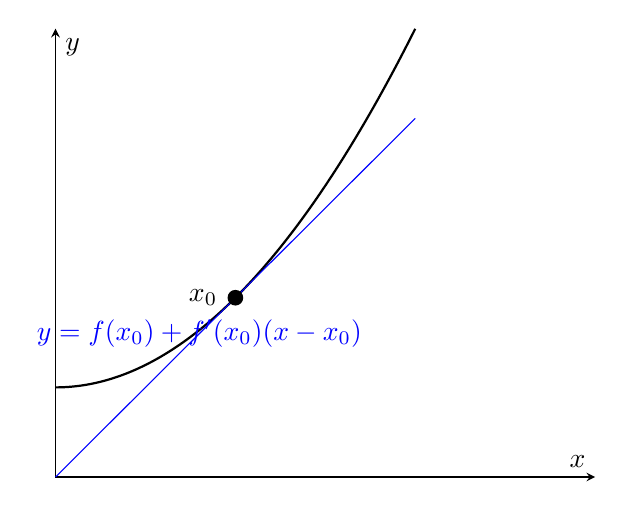
\begin{tikzpicture}
    \begin{axis}[
        axis lines = middle,
        xlabel = \( x \),
        ylabel = \( y \),
        xtick=\empty,
        ytick=\empty,
        clip=false,
        ymin=0,
        ymax=5,
        xmin=0,
        xmax=3
    ]
    
    % Curve equation
    \addplot [domain=0:2, samples=100, smooth, thick] {x^2 + 1};
    
    % Tangent line equation at x0
    \pgfmathsetmacro{\xZero}{1}
    \pgfmathsetmacro{\yZero}{(\xZero)^2 + 1}
    \pgfmathsetmacro{\derivative}{2*\xZero}
    \addplot [domain=0:2, samples=2, smooth, color=blue] {\derivative*(x - \xZero) + \yZero} node[pos=0.4]{$y = f(x_0) + f'(x_0)(x-x_0)$};
    
    % Point of tangency
    \node[label={180:{\( x_0 \)}},circle,fill,inner sep=2pt] at (axis cs:\xZero,\yZero) {};
    
    \end{axis}
    \end{tikzpicture}

$x_0$ is a stationary point of the function $f(x)$ if $f'(x_0) = 0$.
If we use the taylor polynomial
$$f(x) = f(x_0) + f'(x_0)(x-x_0) + \frac{f''(x_0)}{2}(x-x_0)^2 + \ldots$$

We have that
$$f(x) \approx f(x_0) + \frac{f''(x_0)}{2}(x-x_0)^2 + \ldots \quad f'(x_0) = 0 $$

\subsection{Tangent plane}

$$ f(x, y) = x^2y^2 + xy + y $$
$$ \frac{\partial f}{\partial x} = 2xy^2 + y \quad \frac{\partial f}{\partial y} = 2x^2y + x + 1 $$
$$ z = x_0^2y_0^2 + x_0y_0 + y_0 + \frac{\partial f}{\partial x}(x_0, y_0)(x-x_0) + \frac{\partial f}{\partial y}(x_0, y_0)(y-y_0) $$
$$ z = x_0^2y_0^2 + x_0y_0 + y_0 + (2x_0y_0^2 + y_0)(x-x_0) + (2x_0^2y_0 + x_0 + 1)(y-y_0) $$
$z$ is the tangent plane to $(x_0, y_0)$.

\subsection{The normal vector to a surface}
The normal vector to a surface at a point is a vector that is perpendicular to the tangent plane to that surface at the point.
The normal vector to a surface at a point \( (x_0, y_0) \) is given by:
$$ \vec{n} = \nabla f(x_0, y_0) = \begin{pmatrix}
\frac{\partial f}{\partial x}(x_0, y_0) \\
\frac{\partial f}{\partial y}(x_0, y_0) \\
\end{pmatrix} $$
where \( f \) is a function of two variables.


\section{Differentials}
The differential of a function \( f: \mathbb{R}^n \rightarrow \mathbb{R} \) is defined as:
$$ df = \frac{\partial f}{\partial x_1} dx_1 + \frac{\partial f}{\partial x_2} dx_2 + \cdots + \frac{\partial f}{\partial x_n} dx_n $$
where \( dx_i \) is the differential of the \( i \)-th variable \( x_i \).

\section{Artificial Neural Networks}

\subsection{Activation functions}
Activation functions are used to introduce non-linearity in neural networks.
Sigmoid, ReLU, tanh, Leaky ReLU, ELU, Softmax, Swish, etc.

Sigmoid:
$$\sigma(x) = \frac{1}{1+e^{-x}}, \quad \sigma'(x) = \sigma(x)(1-\sigma(x))$$
$$\tanh(x) = \frac{e^x - e^{-x}}{e^x + e^{-x}}, \quad \tanh'(x) = 1 - \tanh^2(x)$$


% \begin{tikzpicture}
% \begin{axis}[
%     axis lines = middle,
%     xlabel = \( x \),
%     ylabel = \( y \),
%     xtick=\empty,
%     ytick=\empty,
%     clip=false,
%     ymin=0,
%     ymax=1,
%     xmin=-5,
%     xmax=5
% ]
% \plot[domain=-5:5, samples=100, smooth, thick] {1/(1+exp(-x))};
% \end{axis}
% \end{tikzpicture}

\section{Direction derivative}
The directional derivative of a multivariate differentiable function along a given vector \( \vec{v} \) at a given point \( \vec{x} \) intuitively represents the instantaneous rate of change of the function, moving through \( \vec{x} \), in the direction of \( \vec{v} \). It therefore generalizes the notion of a partial derivative, in which the rate of change is taken along the direction of one of the coordinate axes, all other coordinates being constant.

The directional derivative of a function \( f: \mathbb{R}^n \rightarrow \mathbb{R} \) at a point \( \vec{x} \) in the direction \( \vec{v} \) is defined as:
$$ D_{\vec{v}} f(\vec{x}) = \lim_{h \rightarrow 0} \frac{f(\vec{x} + h\vec{v}) - f(\vec{x})}{h} $$
if this limit exists. In other words, the directional derivative of \( f \) at \( \vec{x} \) in the direction \( \vec{v} \) is the slope of the tangent line to the curve you get by fixing every variable except \( \vec{v} \) and graphing \( f \) as a function of \( \vec{v} \) alone.

\section{Positive definite matrix}
In linear algebra, a symmetric \( n \times n \) real matrix \( M \) is said to be positive definite if the scalar \( z^TMz \) is strictly positive for every non-zero column vector \( z \) of \( n \) real numbers. Here \( z^T \) denotes the transpose of \( z \).

Let be \( A \in \mathbb{R}^{n \times n} \) a symmetric matrix. \( A \) is positive definite if and only if all its eigenvalues are positive.



\end{document}